\documentclass[DIV16,BCOR1cm,11pt,a4paper,fleqn,twoside]{scrreprt}         % for pdf output
%\documentclass[DIV16,BCOR1cm,11pt,a4paper,fleqn]{report}         % for pdf output

% To allow automatic selection of the right graphics type ...
% preset \pdfoutput for older latex installation, it is allways defined for
% news ones
\ifx\pdfoutput\undefined
\gdef\pdfoutput{0}
\fi

\newif\ifpdfx
\ifnum\pdfoutput=0
% latex is called for dvi output
   \pdfxfalse
   \usepackage{graphics}
   \usepackage{hyperref}
\else
% pdflatex is called for pdf output
   \pdfxtrue
   \usepackage[pdftex]{graphicx}
   \usepackage[pdftex]{hyperref}
\fi

\setlength{\parindent}{0pt}
\usepackage{graphics}

\newcommand{\CDI}{\bfseries\sffamily CDI}

% To define headers and footers
\usepackage{fancyhdr}
\pagestyle{fancy}

% Headers and footers personalization using the `fancyhdr' package
\fancyhf{} % Clear all fields

\renewcommand{\headrulewidth}{0.2mm}
\renewcommand{\footrulewidth}{0.2mm}

\renewcommand{\chaptermark}[1]{\markboth{#1}{}}
%\renewcommand{\sectionmark}[1]{\markright{#1}}

\fancyhead[LO,RE]{\slshape \leftmark}
%\fancyhead[LE,RO]{\slshape \rightmark}
\fancyfoot[LE,RO]{\Large\thepage}
\fancypagestyle{plain}{%
  \fancyhead{} % get rid of headers
  \renewcommand{\headrulewidth}{0pt}
}

\usepackage{html}
\usepackage{exscale}
\usepackage{array,colortbl}    % color table

\usepackage{listings}
%\lstloadlanguages{[ANSI]C,[77]Fortran}
\usepackage{color}
\definecolor{pyellow}{rgb}{1, 0.98, 0.86}

%\usepackage{ae}               % fuer die "almost european" computer modern fonts
%\usepackage{url}              % Standard-Paket fuer WWW-Adressen

%\typearea{10}                 % Einen sinnvollen Satzspiegel aktivieren

%\documentclass[DIV16,BCOR1cm,12pt,a4paper,fleqn]{scrreprt}         % for pdf output
%\documentclass[DIV16,BCOR1cm,11pt,a4paper,twoside]{scrreprt}  % for ps output
%\documentclass[a4paper,DIV14,BCOR1cm]{scrartcl}

%Usage:
%latex2html -local_icons -split 4 -toc_depth 3 -white cdi.tex
%dvips -o cdi.ps cdi.dvi
%dvips ps+pdf
%dvipdf
%pdflatex

\usepackage{thumbpdf}

%\usepackage{html}

\usepackage{makeidx}

%\ifpdf
%\usepackage[a4paper, colorlinks=true, pdfstartview=FitV, bookmarks=true, linkcolor=blue,
%            citecolor=blue, urlcolor=blue, latex2html=true]{hyperref}
%\fi

\usepackage{hyperref}
\hypersetup{pdftoolbar=true,
            pdfmenubar=true,
            pdfwindowui=true,   
%            pdffitwindow=true,
            pdfauthor={Uwe Schulzweida},
            pdftitle={CDI C Manual},
            pdfcreator={pdflatex + hyperref},
            pdfstartview=FitV,
%            pdfpagemode=FullScreen,
            a4paper,
            bookmarks=true,
            linkcolor=blue,
            citecolor=blue,
            urlcolor=blue,
            colorlinks=true}

\makeindex
%\newcommand{\ii}[1]{\textit{#1}}  \newcommand{\nn}[1]{#1n}
%\renewcommand{\dotfill}{\leaders\hbox to 5p1{\hss.\hss}\hfill}
%\newcommand{\idxdotfill}{5p1{\hss.\hss}\hfill}
\newcommand{\idxdotfill}{\ \dotfill \ }
%\def\idxdotfill{\leaders\hbox to.6em{\hss .\hss}\hskip 0pt plus 1fill}
%\MakeShortVerb{\@}

\renewcommand{\indexname}{Function index}


\newcommand{\deflabel}[1]{\bfseries #1\hfill}
\newenvironment{deflist}[1]
{\begin{list}{}
{\settowidth{\labelwidth}{\bfseries #1}
\setlength{\parsep}{0mm}
\setlength{\itemsep}{1mm}
\setlength{\leftmargin}{\labelwidth}
\addtolength{\leftmargin}{\labelsep}
\renewcommand{\makelabel}{\deflabel}}}
{\end{list}}


\begin{document}

\begin{titlepage}
\vspace*{50mm}
{\Huge{\CDI} \ \bfseries C Manual}

\setlength{\unitlength}{1cm}
\begin{picture}(16,0.4)
\linethickness{1.5mm}
\put(0,0.1){\line(1,0){16.3}}
\end{picture}

\begin{flushright}
{\large\bfseries Climate Data Interface \\ Version 2.2.0 \\ March 2023}
\end{flushright}

\vfill

{\Large\bfseries Uwe Schulzweida}

{\Large\bfseries Max-Planck-Institute for Meteorology}

\begin{picture}(16,1)
\linethickness{1.0mm}
\put(0,0.7){\line(1,0){16.3}}
\end{picture}
\end{titlepage}


\tableofcontents


\chapter{Introduction}
The scalability of Earth System Models (ESMs) is the leading target of the 
\href{http://www.dkrz.de/Klimaforschung/dkrz-und-klimaforschung/infraproj/scales
}{ScalES}
project, in particular with regard to future computer development. Our work  
focuses on overcoming the I/O bottleneck.  The 
\href{https://code.mpimet.mpg.de/projects/cdi}{Climate Data Interface} ({\CDI}) is a 
sophisticated data handling library of 
the Max-Planck-Institute for Meteorology with broad acceptence in the 
community. 
\begin{wrapfigure}{r}{.4\textwidth}
\vspace{-10pt}
\centering
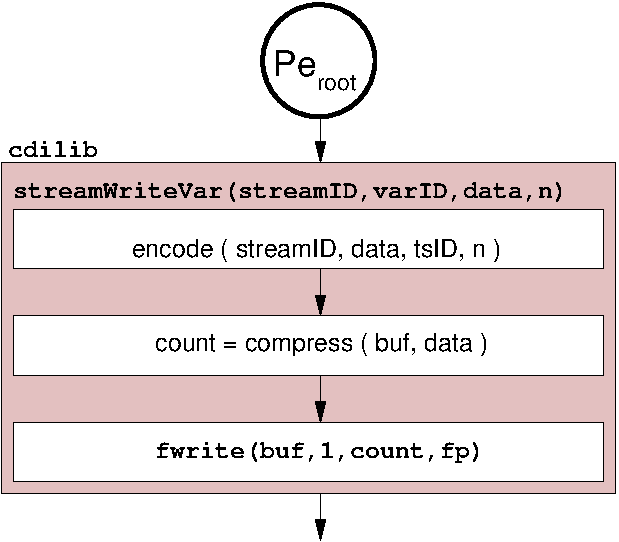
\includegraphics[scale=0.5]{../graphics/serial.pdf}
\vspace{-10pt}
\caption{{{\CDI} {\tt streamWriteVar}}}
\vspace{-10pt}
\end{wrapfigure}
Its I/O is carried out synchronously relative to the model calculation. 
We have decided to parallelize the file writing with the {\CDI}, because of the 
great benefit for many ESMs.
\smallskip 
 
We analyzed 
some HPC systems concerning the impact of their architecture, filesystem and 
MPI implementation on their I/O performance and scalability. The investigation 
delivered a large spectrum of results. As a consequence, 
we introduce different modes of low level file writing. The tasks 
of the I/O processes, which are now decoupled from the model calculation, are split.
We destinguish into collecting the data, encode, compress 
and buffer it on one side and writing the data to file on the other. The extension 
of the {\CDI} with parallel writing ({\pio}) provides five different I/O modes 
making use of this role allocation. The modulation of I/O mode, numbers and 
location of processes with the best performance on a 
special machine can be determined in test runs. 
\smallskip  

On some systems it is impossible to write from different physical nodes to one 
file. Taking the architectural structures into consideration we made a key 
pillar for the design of {\pio} from the distribution of I/O processes and files 
on physical nodes. If the I/O processes are located on different physical nodes, 
the {\tt MPI} communicator for the group of I/O processes is split and each 
subgroup gets a loadbalanced subset of the files to write. On some machines 
this approach increases the throughput remarkably.
\smallskip 

The application programming interface of the {\CDI} is kept untouched, 
we introduce only a few indispensable functions and encapsulate the other 
developments inside the library. The models have to eliminate the special 
position of the root process with respect to file writing. All model processes 
``write'' their chunk of the decomposed data and save the time former needed 
for gathering and low level writing. 


\chapter{File Formats}
%Every input and output file is a collection of 2D or 3D variables
%over an unlimited number of time steps.

\section{GRIB}

GRIB \cite{GRIB} (GRIdded Binary) is a standard format designed by the
World Meteorological Organization (WMO) to support the efficient 
transmission and storage of gridded meteorological data.

A GRIB record consists of a series of header sections, followed by
a bitstream of packed data representing one horizontal grid of data
values. The header sections are intended to fully describe the data
included in the bitstream, specifying information such as the
parameter, units, and precision of the data, the grid system and
level type on which the data is provided, and the date and time
for which the data are valid.

Non-numeric descriptors are enumerated in tables, such that a 1-byte
code in a header section refers to a unique description.
The WMO provides a standard set of enumerated parameter names and
level types, but the standard also allows for the definition
of locally used parameters and geometries. Any activity
that generates and distributes GRIB records must also make
their locally defined GRIB tables available to users.

The GRIB records must be sorted by time to be able to read them correctly with {\CDI}.

{\CDI} does not support the full GRIB standard. The following
data representation and level types are implemented: \\

\begin{tabular}{|r|r|l|l|}
\hline
\rowcolor[gray]{.9}
GRIB1  & GRIB2 & & \\
\rowcolor[gray]{.9}
 grid type &  template & GRIB\_API name & description \\
     0  & 3.0 & regular\_ll & Regular longitude/latitude grid \\
     3  & -- & lambert & Lambert conformal grid \\
     4  & 3.40 & regular\_gg & Regular Gaussian longitude/latitude grid \\
     4  & 3.40 & reduced\_gg & Reduced Gaussian longitude/latitude grid \\
   10  & 3.1 & rotated\_ll & Rotated  longitude/latitude grid \\
   50  & 3.50 & sh & Spherical harmonic coefficients \\
 192  & 3.100 & -- & Icosahedral-hexagonal GME grid \\
  --   & 3.101 & -- & General unstructured grid \\
\hline
\end{tabular}


\begin{tabular}{|r|r|l|l|}
\hline
\rowcolor[gray]{.9}
GRIB1  & GRIB2 & & \\
\rowcolor[gray]{.9}
 level type &  level type & GRIB\_API name & description \\
     1  &    1 & surface                        & Surface level \\
     2  &    2 & cloudBase                    & Cloud base level \\
     3  &    3 & cloudTop                     & Level of cloud tops \\
     4  &    4 & isothermZero               & Level of 0$^{\circ}$ C isotherm \\
     8  &    8 & nominalTop                 & Norminal top of atmosphere \\
     9  &    9 & seaBottom                   & Sea bottom \\
   10  &  10 & entireAtmosphere        & Entire atmosphere \\
 100  & 100 & isobaricInhPa              & Isobaric level in hPa \\
 102  & 101 & meanSea                     & Mean sea level \\
 103  & 102 & heightAboveSea          & Altitude above mean sea level \\
 105  & 103 & heightAboveGround    & Height level above ground \\
 107  & 104 & sigma                          & Sigma level \\
 109  & 105 & hybrid                         & Hybrid level      \\
 110  & 105 & hybridLayer                 & Layer between two hybrid levels   \\
 111  & 106 & depthBelowLand          & Depth below land surface    \\
 112  & 106 & depthBelowLandLayer & Layer between two depths below land surface   \\   
 113  & 107 & theta                           & Isentropic (theta) level \\
   --  & 114 & --                               & Snow level \\
 160  & 160 & depthBelowSea            & Depth below sea level    \\
 162  & 162 & --                               & Lake or River Bottom \\
 163  & 163 & --                               & Bottom Of Sediment Layer  \\
 164  & 164 & --                               & Bottom Of Thermally Active Sediment Layer  \\
 165  & 165 & --                               & Bottom Of Sediment Layer Penetrated By \\ 
         &        &                                    & Thermal Wave  \\
 166  & 166 & --                               & Mixing Layer  \\
 210  & --   & isobaricInPa                & Isobaric level in Pa \\
\hline
\end{tabular}

\subsection{GRIB edition 1}

GRIB1 is implemented in {\CDI} as an internal library and enabled per default.
The internal GRIB1 library is called CGRIBEX. This is a lightweight
version of the ECMWF GRIBEX library. CGRIBEX is written in ANSI C with a portable Fortran interface. 
The configure option \texttt{--disable-cgribex} will disable the encoding/decoding of GRIB1 records with CGRIBEX.

\subsection{GRIB edition 2}

GRIB2 is available in {\CDI} via the ECMWF ecCodes \cite{ecCodes} library.
ecCodes is an external library and not part of {\CDI}. To use GRIB2 with
{\CDI} the ecCodes library must be installed before the configuration
of the {\CDI} library. Use the configure option \texttt{--with-eccodes} to
enable GRIB2 support. 

The ecCodes library is also used to encode/decode GRIB1 records if the support for the CGRIBEX library is disabled.
This feature is not tested regulary and the status is experimental!

A single GRIB2 message can contain multiple fields. This feature is not supported in {\CDI}!

\section{NetCDF}

NetCDF \cite{NetCDF} (Network Common Data Form) is an interface for array-oriented data
access and a library that provides an implementation of the interface.
The NetCDF library also defines a machine-independent format for 
representing scientific data. Together, the interface, library, and 
format support the creation, access, and sharing of scientific data.

{\CDI} only supports the classic data model of NetCDF and arrays up to 4 dimensions.
These dimensions should only be used by the horizontal and vertical grid and the time.
The NetCDF attributes should follow the
\href{http://ftp.unidata.ucar.edu/software/netcdf/docs/conventions.html}
     {GDT, COARDS or CF Conventions}.

NetCDF is an external library and not part of {\CDI}. To use NetCDF with
{\CDI} the NetCDF library must be installed before the configuration
of the {\CDI} library. Use the configure option \texttt{--with-netcdf} to
enable NetCDF support (see \htmlref{Build}{build}).

%\subsection{ncdap}


\section{SERVICE}

SERVICE is the binary exchange format of the atmospheric general circulation model ECHAM \cite{ECHAM}.
It has a header section with 8 integer values followed by the data section.
The header and the data section have the standard Fortran blocking for binary data records.
A SERVICE record can have an accuracy of 4 or 8 bytes and the byteorder can be little or big endian.
In {\CDI} the accuracy of the header and data section must be the same.
The following Fortran code example can be used to read a SERVICE record with an accuracy of 4 bytes:

\begin{lstlisting}[language=Fortran, backgroundcolor=\color{pyellow}, basicstyle=\small, columns=flexible]
   INTEGER*4 icode,ilevel,idate,itime,nlon,nlat,idispo1,idispo2
   REAL*4 field(mlon,mlat)
      ...
   READ(unit) icode,ilevel,idate,itime,nlon,nlat,idispo1,idispo2
   READ(unit) ((field(ilon,ilat), ilon=1,nlon), ilat=1,nlat)
\end{lstlisting}

The constants \texttt{mlon} and \texttt{mlat} must be greater or equal than \texttt{nlon} and \texttt{nlat}.
The meaning of the variables are:

\vspace*{3mm}
\hspace*{8mm}\begin{minipage}{10cm}
\begin{deflist}{\texttt{idispo2 \ \ }}
\item[\texttt{icode}]    The code number
\item[\texttt{ilevel}]   The level
\item[\texttt{idate}]    The date as YYYYMMDD
\item[\texttt{itime}]    The time as hhmmss
\item[\texttt{nlon}]     The number of longitudes
\item[\texttt{nlat}]     The number of latitides
\item[\texttt{idispo1}]  For the users disposal (Not used in {\CDI})
\item[\texttt{idispo2}]  For the users disposal (Not used in {\CDI})
\end{deflist}
\end{minipage}
\vspace*{3mm}

SERVICE is implemented in {\CDI} as an internal library and enabled per default.
The configure option \texttt{--disable-service} will disable the support for the SERVICE format.

\section{EXTRA}

EXTRA is the standard binary output format of the ocean model MPIOM \cite{MPIOM}.
It has a header section with 4 integer values followed by the data section. 
The header and the data section have the standard Fortran blocking for binary data records.
An EXTRA record can have an accuracy of 4 or 8 bytes and the byteorder can be little or big endian.
In {\CDI} the accuracy of the header and data section must be the same.
The following Fortran code example can be used to read an EXTRA record with an accuracy of 4 bytes:

\begin{lstlisting}[language=Fortran, backgroundcolor=\color{pyellow}, basicstyle=\small, columns=flexible]
   INTEGER*4 idate,icode,ilevel,nsize
   REAL*4 field(msize)
      ...
   READ(unit) idate,icode,ilevel,nsize
   READ(unit) (field(isize),isize=1,nsize)
\end{lstlisting}

The constant \texttt{msize} must be greater or equal than \texttt{nsize}.
The meaning of the variables are:

\vspace*{3mm}
\hspace*{8mm}\begin{minipage}{10cm}
\begin{deflist}{\texttt{idispo2 \ \ }}
\item[\texttt{idate}]    The date as YYYYMMDD
\item[\texttt{icode}]    The code number
\item[\texttt{ilevel}]   The level
\item[\texttt{nsize}]    The size of the field
\end{deflist}
\end{minipage}
\vspace*{3mm}

EXTRA is implemented in {\CDI} as an internal library and enabled per default.
The configure option \texttt{--disable-extra} will disable the support for the EXTRA format.


\section{IEG}

IEG is the standard binary output format of the regional model REMO \cite{REMO}.
It is simple an unpacked GRIB edition 1 format. The product and grid
description sections are coded with 4 byte integer values and the
data section can have 4 or 8 byte IEEE floating point values.
The header and the data section have the standard Fortran blocking
for binary data records. The IEG format has a fixed size of 100 for the
vertical coordinate table. That means it is not possible to store more
than 50 model levels with this format.
{\CDI} supports only data on Gaussian and LonLat grids for the IEG format.

IEG is implemented in {\CDI} as an internal library and enabled per default.
The configure option \texttt{--disable-ieg} will disable the support for the IEG format.



\chapter{Use of the CDI Library}
This chapter provides templates of common sequences of {\CDI} calls needed for common uses.
For clarity only the names of routines are used. Declarations and error checking were omitted.
Statements that are typically invoked multiple times were indented and ... is used to 
represent arbitrary sequences of other statements. 
Full parameter lists are described in later chapters.

Complete examples for write, read and copy a dataset with {\CDI}
can be found in \htmlref{Appendix B}{example}.

\section{Creating a dataset}

Here is a typical sequence of {\CDI} calls used to create a new dataset:

\begin{lstlisting}[backgroundcolor=\color{pyellow}, basicstyle=\small]
    gridCreate           ! create a horizontal Grid: from type and size
       ...
    zaxisCreate          ! create a vertical Z-axis: from type and size
       ...
    taxisCreate          ! create a Time axis: from type
       ...
    vlistCreate          ! create a variable list
          ...
       vlistDefVar       ! define variables: from Grid and Z-axis
          ...
    streamOpenWrite      ! create a dataset: from name and file type
       ...
    streamDefVlist       ! define variable list
       ...
    streamDefTimestep    ! define time step
          ...   
       streamWriteVar    ! write variable
          ...
    streamClose          ! close the dataset
       ...
    vlistDestroy         ! destroy the variable list
       ...
    taxisDestroy         ! destroy the Time axis
       ...
    zaxisDestroy         ! destroy the Z-axis
       ...
    gridDestroy          ! destroy the Grid
\end{lstlisting}


\section{Reading a dataset}

Here is a typical sequence of {\CDI} calls used to read a dataset:

\begin{lstlisting}[backgroundcolor=\color{pyellow}, basicstyle=\small]
    streamOpenRead       ! open existing dataset
       ...
    streamInqVlist       ! find out what is in it
          ...
       vlistInqVarGrid   ! get an identifier to the Grid
          ...
       vlistInqVarZaxis  ! get an identifier to the Z-axis
          ...
       vlistInqTaxis     ! get an identifier to the T-axis
          ...
    streamInqTimestep    ! get time step
          ...
       streamReadVar     ! read varible
          ...
    streamClose          ! close the dataset
\end{lstlisting}


\section{Compiling and Linking with the CDI library}

Details of how to compile and link a program that uses the {\CDI} C or FORTRAN
interfaces differ, depending on the operating system, the available compilers,
and where the {\CDI} library and include files are installed.
Here are examples of how to compile and link a program that uses the {\CDI} library
on a Unix platform, so that you can adjust these examples to fit your installation.

Every C file that references {\CDI} functions or constants must contain
an appropriate \texttt{include} statement before the first such reference:

\begin{verbatim}
   #include "cdi.h"
\end{verbatim}

Unless the \texttt{cdi.h} file is installed in a standard directory where
C compiler always looks, you must use the \texttt{-I} option when invoking
the compiler, to specify a directory where \texttt{cdi.h} is installed, for example:

\begin{verbatim}
   cc -c -I/usr/local/cdi/include myprogram.c
\end{verbatim}

Alternatively, you could specify an absolute path name in the \texttt{include}
statement, but then your program would not compile on another platform
where {\CDI} is installed in a different location.

Unless the {\CDI} library is installed in a standard directory where the linker
always looks, you must use the \texttt{-L} and \texttt{-l} options to links an object file that
uses the {\CDI} library. For example:

\begin{verbatim}
   cc -o myprogram myprogram.o -L/usr/local/cdi/lib -lcdi -lm
\end{verbatim}

Alternatively, you could specify an absolute path name for the library:

\begin{verbatim}
   cc -o myprogram myprogram.o -L/usr/local/cdi/lib/libcdi -lm
\end{verbatim}

If the {\CDI} library is using other external libraries, you must add this
libraries in the same way.
For example with the NetCDF library:

\begin{verbatim}
   cc -o myprogram myprogram.o -L/usr/local/cdi/lib -lcdi -lm \
                               -L/usr/local/netcdf/lib -lnetcdf
\end{verbatim}



\chapter{CDI modules}
%Complete examples for write, read and copy a dataset with {\CDI}
%can be found in \htmlref{Appendix B}{example}.


%\newpage
\section{Dataset functions}
This module contains functions to read and write the data.
To create a new dataset the output format must be specified
with one of the following predefined file format types:

\vspace*{3mm}
\hspace*{8mm}\begin{minipage}{15cm}
\begin{deflist}{\large\texttt{CDI\_FILETYPE\_GRB2 \ \ }}
\item[{\large\texttt{CDI\_FILETYPE\_GRB}}]   File type GRIB version 1
\item[{\large\texttt{CDI\_FILETYPE\_GRB2}}]  File type GRIB version 2          
\item[{\large\texttt{CDI\_FILETYPE\_NC }}]   File type NetCDF
\item[{\large\texttt{CDI\_FILETYPE\_NC2}}]   File type NetCDF version 2 (64-bit offset)
\item[{\large\texttt{CDI\_FILETYPE\_NC4}}]   File type NetCDF-4 (HDF5)
\item[{\large\texttt{CDI\_FILETYPE\_NC4C}}]  File type NetCDF-4 classic
\item[{\large\texttt{CDI\_FILETYPE\_NC5}}]   File type NetCDF version 5 (64-bit data)
\item[{\large\texttt{CDI\_FILETYPE\_NCZARR}}]   File type NetCDF NCZarr
\item[{\large\texttt{CDI\_FILETYPE\_SRV}}]   File type SERVICE
\item[{\large\texttt{CDI\_FILETYPE\_EXT}}]   File type EXTRA
\item[{\large\texttt{CDI\_FILETYPE\_IEG}}]   File type IEG
\end{deflist}
\end{minipage}
\vspace*{3mm}

\texttt{CDI\_FILETYPE\_GRB2} is only available if the {\CDI} library was compiled with ecCodes support and all NetCDF file types are only available if the {\CDI} library was compiled with NetCDF support!

To set the byte order of a binary dataset with the file format
type \texttt{CDI\_FILETYPE\_SRV}, \texttt{CDI\_FILETYPE\_EXT} or \texttt{CDI\_FILETYPE\_IEG} use one of the
following predefined constants in the call to {\htmlref{\texttt{streamDefByteorder}}{streamDefByteorder}}:

\vspace*{3mm}
\hspace*{8mm}\begin{minipage}{15cm}
\begin{deflist}{\large\texttt{CDI\_LITTLEENDIAN \ \ }}
\item[{\large\texttt{CDI\_BIGENDIAN   }}]  Byte order big endian
\item[{\large\texttt{CDI\_LITTLEENDIAN}}]  Byte order little endian
\end{deflist}
\end{minipage}
\vspace*{3mm}



\subsection{Create a new dataset: \texttt{streamOpenWrite}}
\index{streamOpenWrite}
\label{streamOpenWrite}

The function {\texttt{streamOpenWrite}} creates a new datset.
\subsubsection*{Usage}

\begin{verbatim}
    int streamOpenWrite(const char *path, int filetype);
\end{verbatim}

\hspace*{4mm}\begin{minipage}[]{15cm}
\begin{deflist}{\texttt{filetype}\ }
\item[\texttt{path}]
The name of the new dataset.
\item[\texttt{filetype}]
The type of the file format, one of the set of predefined {\CDI} file format types.
                     The valid {\CDI} file format types are {\texttt{CDI\_FILETYPE\_GRB}}, {\texttt{CDI\_FILETYPE\_GRB2}}, {\texttt{CDI\_FILETYPE\_NC}},
                     {\texttt{CDI\_FILETYPE\_NC2}}, {\texttt{CDI\_FILETYPE\_NC4}}, {\texttt{CDI\_FILETYPE\_NC4C}}, {\texttt{CDI\_FILETYPE\_NC5}},
                     {\texttt{CDI\_FILETYPE\_NCZARR}}, {\texttt{CDI\_FILETYPE\_SRV}}, {\texttt{CDI\_FILETYPE\_EXT}} and {\texttt{CDI\_FILETYPE\_IEG}}.

\end{deflist}
\end{minipage}

\subsubsection*{Result}

Upon successful completion {\texttt{streamOpenWrite}} returns an identifier to the
open stream. Otherwise, a negative number with the error status is returned.


\subsubsection*{Errors}


\hspace*{4mm}\begin{minipage}[]{15cm}
\begin{deflist}{\texttt{CDI\_EUFILETYPE}\ }
\item[\texttt{CDI\_ESYSTEM}]
Operating system error.
\item[\texttt{CDI\_EINVAL}]
Invalid argument.
\item[\texttt{CDI\_EUFILETYPE}]
Unsupported file type.
\item[\texttt{CDI\_ELIBNAVAIL}]
Library support not compiled in.
\end{deflist}
\end{minipage}


\subsubsection*{Example}

Here is an example using {\texttt{streamOpenWrite}} to create a new NetCDF file named {\texttt{foo.nc}} for writing:

\begin{lstlisting}[language=C, backgroundcolor=\color{pyellow}, basicstyle=\small, columns=flexible]

    #include "cdi.h"
       ...
    int streamID;
       ...
    streamID = streamOpenWrite("foo.nc", CDI_FILETYPE_NC);
    if ( streamID < 0 ) handle_error(streamID);
       ...
\end{lstlisting}


\subsection{Open a dataset for reading: \texttt{streamOpenRead}}
\index{streamOpenRead}
\label{streamOpenRead}

The function {\texttt{streamOpenRead}} opens an existing dataset for reading.

\subsubsection*{Usage}

\begin{verbatim}
    int streamOpenRead(const char *path);
\end{verbatim}

\hspace*{4mm}\begin{minipage}[]{15cm}
\begin{deflist}{\texttt{path}\ }
\item[\texttt{path}]
The name of the dataset to be read.

\end{deflist}
\end{minipage}

\subsubsection*{Result}

Upon successful completion {\texttt{streamOpenRead}} returns an identifier to the
open stream. Otherwise, a negative number with the error status is returned.


\subsubsection*{Errors}


\hspace*{4mm}\begin{minipage}[]{15cm}
\begin{deflist}{\texttt{CDI\_EUFILETYPE}\ }
\item[\texttt{CDI\_ESYSTEM}]
Operating system error.
\item[\texttt{CDI\_EINVAL}]
Invalid argument.
\item[\texttt{CDI\_EUFILETYPE}]
Unsupported file type.
\item[\texttt{CDI\_ELIBNAVAIL}]
Library support not compiled in.
\end{deflist}
\end{minipage}


\subsubsection*{Example}

Here is an example using {\texttt{streamOpenRead}} to open an existing NetCDF
file named {\texttt{foo.nc}} for reading:

\begin{lstlisting}[language=C, backgroundcolor=\color{pyellow}, basicstyle=\small, columns=flexible]

    #include "cdi.h"
       ...
    int streamID;
       ...
    streamID = streamOpenRead("foo.nc");
    if ( streamID < 0 ) handle_error(streamID);
       ...
\end{lstlisting}


\subsection{Close an open dataset: \texttt{streamClose}}
\index{streamClose}
\label{streamClose}

The function {\texttt{streamClose}} closes an open dataset.

\subsubsection*{Usage}

\begin{verbatim}
    void streamClose(int streamID);
\end{verbatim}

\hspace*{4mm}\begin{minipage}[]{15cm}
\begin{deflist}{\texttt{streamID}\ }
\item[\texttt{streamID}]
Stream ID, from a previous call to {\htmlref{\texttt{streamOpenRead}}{streamOpenRead}} or {\htmlref{\texttt{streamOpenWrite}}{streamOpenWrite}}.

\end{deflist}
\end{minipage}


\subsection{Get the filetype: \texttt{streamInqFiletype}}
\index{streamInqFiletype}
\label{streamInqFiletype}

The function {\texttt{streamInqFiletype}} returns the filetype of a stream.

\subsubsection*{Usage}

\begin{verbatim}
    int streamInqFiletype(int streamID);
\end{verbatim}

\hspace*{4mm}\begin{minipage}[]{15cm}
\begin{deflist}{\texttt{streamID}\ }
\item[\texttt{streamID}]
Stream ID, from a previous call to {\htmlref{\texttt{streamOpenRead}}{streamOpenRead}} or {\htmlref{\texttt{streamOpenWrite}}{streamOpenWrite}}.

\end{deflist}
\end{minipage}

\subsubsection*{Result}

{\texttt{streamInqFiletype}} returns the type of the file format,
one of the set of predefined {\CDI} file format types.
The valid {\CDI} file format types are {\texttt{CDI\_FILETYPE\_GRB}}, {\texttt{CDI\_FILETYPE\_GRB2}}, {\texttt{CDI\_FILETYPE\_NC}},
{\texttt{CDI\_FILETYPE\_NC2}}, {\texttt{CDI\_FILETYPE\_NC4}}, {\texttt{CDI\_FILETYPE\_NC4C}}, {\texttt{CDI\_FILETYPE\_NC5}},
{\texttt{CDI\_FILETYPE\_NCZARR}}, {\texttt{CDI\_FILETYPE\_SRV}}, {\texttt{CDI\_FILETYPE\_EXT}} and {\texttt{CDI\_FILETYPE\_IEG}}.


\subsection{Define the byte order: \texttt{streamDefByteorder}}
\index{streamDefByteorder}
\label{streamDefByteorder}

The function {\texttt{streamDefByteorder}} defines the byte order of a binary dataset
with the file format type {\texttt{CDI\_FILETYPE\_SRV}}, {\texttt{CDI\_FILETYPE\_EXT}} or {\texttt{CDI\_FILETYPE\_IEG}}.

\subsubsection*{Usage}

\begin{verbatim}
    void streamDefByteorder(int streamID, int byteorder);
\end{verbatim}

\hspace*{4mm}\begin{minipage}[]{15cm}
\begin{deflist}{\texttt{byteorder}\ }
\item[\texttt{streamID}]
Stream ID, from a previous call to {\htmlref{\texttt{streamOpenWrite}}{streamOpenWrite}}.
\item[\texttt{byteorder}]
The byte order of a dataset, one of the {\CDI} constants {\texttt{CDI\_BIGENDIAN}} and
                     {\texttt{CDI\_LITTLEENDIAN}}.

\end{deflist}
\end{minipage}


\subsection{Get the byte order: \texttt{streamInqByteorder}}
\index{streamInqByteorder}
\label{streamInqByteorder}

The function {\texttt{streamInqByteorder}} returns the byte order of a binary dataset
with the file format type {\texttt{CDI\_FILETYPE\_SRV}}, {\texttt{CDI\_FILETYPE\_EXT}} or {\texttt{CDI\_FILETYPE\_IEG}}.

\subsubsection*{Usage}

\begin{verbatim}
    int streamInqByteorder(int streamID);
\end{verbatim}

\hspace*{4mm}\begin{minipage}[]{15cm}
\begin{deflist}{\texttt{streamID}\ }
\item[\texttt{streamID}]
Stream ID, from a previous call to {\htmlref{\texttt{streamOpenRead}}{streamOpenRead}} or {\htmlref{\texttt{streamOpenWrite}}{streamOpenWrite}}.

\end{deflist}
\end{minipage}

\subsubsection*{Result}

{\texttt{streamInqByteorder}} returns the type of the byte order.
The valid {\CDI} byte order types are {\texttt{CDI\_BIGENDIAN}} and {\texttt{CDI\_LITTLEENDIAN}}



\subsection{Define the variable list: \texttt{streamDefVlist}}
\index{streamDefVlist}
\label{streamDefVlist}

The function {\texttt{streamDefVlist}} defines the variable list of a stream.

To safeguard against errors by modifying the wrong vlist object,
this function makes the passed vlist object immutable.
All further vlist changes have to use the vlist object returned by streamInqVlist().

\subsubsection*{Usage}

\begin{verbatim}
    void streamDefVlist(int streamID, int vlistID);
\end{verbatim}

\hspace*{4mm}\begin{minipage}[]{15cm}
\begin{deflist}{\texttt{streamID}\ }
\item[\texttt{streamID}]
Stream ID, from a previous call to {\htmlref{\texttt{streamOpenWrite}}{streamOpenWrite}}.
\item[\texttt{vlistID}]
Variable list ID, from a previous call to {\htmlref{\texttt{vlistCreate}}{vlistCreate}}.

\end{deflist}
\end{minipage}


\subsection{Get the variable list: \texttt{streamInqVlist}}
\index{streamInqVlist}
\label{streamInqVlist}

The function {\texttt{streamInqVlist}} returns the variable list of a stream.

\subsubsection*{Usage}

\begin{verbatim}
    int streamInqVlist(int streamID);
\end{verbatim}

\hspace*{4mm}\begin{minipage}[]{15cm}
\begin{deflist}{\texttt{streamID}\ }
\item[\texttt{streamID}]
Stream ID, from a previous call to {\htmlref{\texttt{streamOpenRead}}{streamOpenRead}} or {\htmlref{\texttt{streamOpenWrite}}{streamOpenWrite}}.

\end{deflist}
\end{minipage}

\subsubsection*{Result}

{\texttt{streamInqVlist}} returns an identifier to the variable list.



\subsection{Define a timestep: \texttt{streamDefTimestep}}
\index{streamDefTimestep}
\label{streamDefTimestep}

The function {\texttt{streamDefTimestep}} defines a timestep of a stream by the identifier tsID.
The identifier tsID is the timestep index starting at 0 for the first timestep.
Before calling this function the functions {\texttt{taxisDefVdate}} and {\texttt{taxisDefVtime}} should be used
to define the timestamp for this timestep. All calls to write the data refer to this timestep.

\subsubsection*{Usage}

\begin{verbatim}
    int streamDefTimestep(int streamID, int tsID);
\end{verbatim}

\hspace*{4mm}\begin{minipage}[]{15cm}
\begin{deflist}{\texttt{streamID}\ }
\item[\texttt{streamID}]
Stream ID, from a previous call to {\htmlref{\texttt{streamOpenWrite}}{streamOpenWrite}}.
\item[\texttt{tsID}]
Timestep identifier.

\end{deflist}
\end{minipage}

\subsubsection*{Result}

{\texttt{streamDefTimestep}} returns the number of expected records of the timestep.



\subsection{Get timestep information: \texttt{streamInqTimestep}}
\index{streamInqTimestep}
\label{streamInqTimestep}

The function {\texttt{streamInqTimestep}} sets the next timestep to the identifier tsID.
The identifier tsID is the timestep index starting at 0 for the first timestep.
After a call to this function the functions {\texttt{taxisInqVdate}} and {\texttt{taxisInqVtime}} can be used
to read the timestamp for this timestep. All calls to read the data refer to this timestep.

\subsubsection*{Usage}

\begin{verbatim}
    int streamInqTimestep(int streamID, int tsID);
\end{verbatim}

\hspace*{4mm}\begin{minipage}[]{15cm}
\begin{deflist}{\texttt{streamID}\ }
\item[\texttt{streamID}]
Stream ID, from a previous call to {\htmlref{\texttt{streamOpenRead}}{streamOpenRead}} or {\htmlref{\texttt{streamOpenWrite}}{streamOpenWrite}}.
\item[\texttt{tsID}]
Timestep identifier.

\end{deflist}
\end{minipage}

\subsubsection*{Result}

{\texttt{streamInqTimestep}} returns the number of records of the timestep or 0, if the end of the file is reached.




\subsection{Write a variable: \texttt{streamWriteVar}}
\index{streamWriteVar}
\label{streamWriteVar}

The function streamWriteVar writes the values of one time step of a variable to an open dataset.
The values are converted to the external data type of the variable, if necessary.
\subsubsection*{Usage}

\begin{verbatim}
    void streamWriteVar(int streamID, int varID, const double *data, SizeType nmiss);
\end{verbatim}

\hspace*{4mm}\begin{minipage}[]{15cm}
\begin{deflist}{\texttt{streamID}\ }
\item[\texttt{streamID}]
Stream ID, from a previous call to {\htmlref{\texttt{streamOpenWrite}}{streamOpenWrite}}.
\item[\texttt{varID}]
Variable identifier.
\item[\texttt{data}]
Pointer to a block of double precision floating point data values to be written.
\item[\texttt{nmiss}]
Number of missing values.

\end{deflist}
\end{minipage}


\subsection{Write a variable: \texttt{streamWriteVarF}}
\index{streamWriteVarF}
\label{streamWriteVarF}

The function streamWriteVarF writes the values of one time step of a variable to an open dataset.
The values are converted to the external data type of the variable, if necessary.
\subsubsection*{Usage}

\begin{verbatim}
    void streamWriteVarF(int streamID, int varID, const float *data, SizeType nmiss);
\end{verbatim}

\hspace*{4mm}\begin{minipage}[]{15cm}
\begin{deflist}{\texttt{streamID}\ }
\item[\texttt{streamID}]
Stream ID, from a previous call to {\htmlref{\texttt{streamOpenWrite}}{streamOpenWrite}}.
\item[\texttt{varID}]
Variable identifier.
\item[\texttt{data}]
Pointer to a block of single precision floating point data values to be written.
\item[\texttt{nmiss}]
Number of missing values.

\end{deflist}
\end{minipage}


\subsection{Write a horizontal slice of a variable: \texttt{streamWriteVarSlice}}
\index{streamWriteVarSlice}
\label{streamWriteVarSlice}

The function streamWriteVarSlice writes the values of a horizontal slice of a variable to an open dataset.
The values are converted to the external data type of the variable, if necessary.
\subsubsection*{Usage}

\begin{verbatim}
    void streamWriteVarSlice(int streamID, int varID, int levelID, const double *data, 
                             SizeType nmiss);
\end{verbatim}

\hspace*{4mm}\begin{minipage}[]{15cm}
\begin{deflist}{\texttt{streamID}\ }
\item[\texttt{streamID}]
Stream ID, from a previous call to {\htmlref{\texttt{streamOpenWrite}}{streamOpenWrite}}.
\item[\texttt{varID}]
Variable identifier.
\item[\texttt{levelID}]
Level identifier.
\item[\texttt{data}]
Pointer to a block of double precision floating point data values to be written.
\item[\texttt{nmiss}]
Number of missing values.

\end{deflist}
\end{minipage}


\subsection{Write a horizontal slice of a variable: \texttt{streamWriteVarSliceF}}
\index{streamWriteVarSliceF}
\label{streamWriteVarSliceF}

The function streamWriteVarSliceF writes the values of a horizontal slice of a variable to an open dataset.
The values are converted to the external data type of the variable, if necessary.
\subsubsection*{Usage}

\begin{verbatim}
    void streamWriteVarSliceF(int streamID, int varID, int levelID, const float *data, 
                              SizeType nmiss);
\end{verbatim}

\hspace*{4mm}\begin{minipage}[]{15cm}
\begin{deflist}{\texttt{streamID}\ }
\item[\texttt{streamID}]
Stream ID, from a previous call to {\htmlref{\texttt{streamOpenWrite}}{streamOpenWrite}}.
\item[\texttt{varID}]
Variable identifier.
\item[\texttt{levelID}]
Level identifier.
\item[\texttt{data}]
Pointer to a block of single precision floating point data values to be written.
\item[\texttt{nmiss}]
Number of missing values.

\end{deflist}
\end{minipage}



\subsection{Read a variable: \texttt{streamReadVar}}
\index{streamReadVar}
\label{streamReadVar}

The function streamReadVar reads all the values of one time step of a variable
from an open dataset.
\subsubsection*{Usage}

\begin{verbatim}
    void streamReadVar(int streamID, int varID, double *data, SizeType *nmiss);
\end{verbatim}

\hspace*{4mm}\begin{minipage}[]{15cm}
\begin{deflist}{\texttt{streamID}\ }
\item[\texttt{streamID}]
Stream ID, from a previous call to {\htmlref{\texttt{streamOpenRead}}{streamOpenRead}}.
\item[\texttt{varID}]
Variable identifier.
\item[\texttt{data}]
Pointer to the location into which the data values are read.
                     The caller must allocate space for the returned values.
\item[\texttt{nmiss}]
Number of missing values.

\end{deflist}
\end{minipage}


\subsection{Read a variable: \texttt{streamReadVarF}}
\index{streamReadVarF}
\label{streamReadVarF}

The function streamReadVar reads all the values of one time step of a variable
from an open dataset.
\subsubsection*{Usage}

\begin{verbatim}
    void streamReadVar(int streamID, int varID, float *data, SizeType *nmiss);
\end{verbatim}

\hspace*{4mm}\begin{minipage}[]{15cm}
\begin{deflist}{\texttt{streamID}\ }
\item[\texttt{streamID}]
Stream ID, from a previous call to {\htmlref{\texttt{streamOpenRead}}{streamOpenRead}}.
\item[\texttt{varID}]
Variable identifier.
\item[\texttt{data}]
Pointer to the location into which the data values are read.
                     The caller must allocate space for the returned values.
\item[\texttt{nmiss}]
Number of missing values.

\end{deflist}
\end{minipage}


\subsection{Read a horizontal slice of a variable: \texttt{streamReadVarSlice}}
\index{streamReadVarSlice}
\label{streamReadVarSlice}

The function streamReadVarSlice reads all the values of a horizontal slice of a variable
from an open dataset.
\subsubsection*{Usage}

\begin{verbatim}
    void streamReadVarSlice(int streamID, int varID, int levelID, double *data, 
                            SizeType *nmiss);
\end{verbatim}

\hspace*{4mm}\begin{minipage}[]{15cm}
\begin{deflist}{\texttt{streamID}\ }
\item[\texttt{streamID}]
Stream ID, from a previous call to {\htmlref{\texttt{streamOpenRead}}{streamOpenRead}}.
\item[\texttt{varID}]
Variable identifier.
\item[\texttt{levelID}]
Level identifier.
\item[\texttt{data}]
Pointer to the location into which the data values are read.
                     The caller must allocate space for the returned values.
\item[\texttt{nmiss}]
Number of missing values.

\end{deflist}
\end{minipage}


\subsection{Read a horizontal slice of a variable: \texttt{streamReadVarSliceF}}
\index{streamReadVarSliceF}
\label{streamReadVarSliceF}

The function streamReadVarSliceF reads all the values of a horizontal slice of a variable
from an open dataset.
\subsubsection*{Usage}

\begin{verbatim}
    void streamReadVarSliceF(int streamID, int varID, int levelID, float *data, 
                             SizeType *nmiss);
\end{verbatim}

\hspace*{4mm}\begin{minipage}[]{15cm}
\begin{deflist}{\texttt{streamID}\ }
\item[\texttt{streamID}]
Stream ID, from a previous call to {\htmlref{\texttt{streamOpenRead}}{streamOpenRead}}.
\item[\texttt{varID}]
Variable identifier.
\item[\texttt{levelID}]
Level identifier.
\item[\texttt{data}]
Pointer to the location into which the data values are read.
                     The caller must allocate space for the returned values.
\item[\texttt{nmiss}]
Number of missing values.

\end{deflist}
\end{minipage}



\newpage
\section{Variable list functions}
This module contains functions to handle a list of variables.
A variable list is a collection of all variables of a dataset.



\subsection{Create a variable list: \texttt{vlistCreate}}
\index{vlistCreate}
\label{vlistCreate}
\subsubsection*{Usage}

\begin{verbatim}
    int vlistCreate(void);
\end{verbatim}

\subsubsection*{Example}

Here is an example using {\texttt{vlistCreate}} to create a variable list
and add a variable with {\texttt{vlistDefVar}}.

\begin{lstlisting}[language=C, backgroundcolor=\color{pyellow}, basicstyle=\small, columns=flexible]

    #include "cdi.h"
       ...
    int vlistID, varID;
       ...
    vlistID = vlistCreate();
    varID = vlistDefVar(vlistID, gridID, zaxisID, TIME_VARYING);
       ...
    streamDefVlist(streamID, vlistID);
       ...
    vlistDestroy(vlistID);
       ...
\end{lstlisting}


\subsection{Destroy a variable list: \texttt{vlistDestroy}}
\index{vlistDestroy}
\label{vlistDestroy}
\subsubsection*{Usage}

\begin{verbatim}
    void vlistDestroy(int vlistID);
\end{verbatim}

\hspace*{4mm}\begin{minipage}[]{15cm}
\begin{deflist}{\texttt{vlistID}\ }
\item[\texttt{vlistID}]
Variable list ID, from a previous call to {\htmlref{\texttt{vlistCreate}}{vlistCreate}}.

\end{deflist}
\end{minipage}


\subsection{Copy a variable list: \texttt{vlistCopy}}
\index{vlistCopy}
\label{vlistCopy}

The function {\texttt{vlistCopy}} copies all entries from vlistID1 to vlistID2.

\subsubsection*{Usage}

\begin{verbatim}
    void vlistCopy(int vlistID2, int vlistID1);
\end{verbatim}

\hspace*{4mm}\begin{minipage}[]{15cm}
\begin{deflist}{\texttt{vlistID2}\ }
\item[\texttt{vlistID2}]
Target variable list ID.
\item[\texttt{vlistID1}]
Source variable list ID.

\end{deflist}
\end{minipage}


\subsection{Duplicate a variable list: \texttt{vlistDuplicate}}
\index{vlistDuplicate}
\label{vlistDuplicate}

The function {\texttt{vlistDuplicate}} duplicates the variable list from vlistID1.

\subsubsection*{Usage}

\begin{verbatim}
    int vlistDuplicate(int vlistID);
\end{verbatim}

\hspace*{4mm}\begin{minipage}[]{15cm}
\begin{deflist}{\texttt{vlistID}\ }
\item[\texttt{vlistID}]
Variable list ID, from a previous call to {\htmlref{\texttt{vlistCreate}}{vlistCreate}} or {\htmlref{\texttt{streamInqVlist}}{streamInqVlist}}.

\end{deflist}
\end{minipage}

\subsubsection*{Result}

{\texttt{vlistDuplicate}} returns an identifier to the duplicated variable list.



\subsection{Concatenate two variable lists: \texttt{vlistCat}}
\index{vlistCat}
\label{vlistCat}

Concatenate the variable list vlistID1 at the end of vlistID2.

\subsubsection*{Usage}

\begin{verbatim}
    void vlistCat(int vlistID2, int vlistID1);
\end{verbatim}

\hspace*{4mm}\begin{minipage}[]{15cm}
\begin{deflist}{\texttt{vlistID2}\ }
\item[\texttt{vlistID2}]
Target variable list ID.
\item[\texttt{vlistID1}]
Source variable list ID.

\end{deflist}
\end{minipage}


\subsection{Copy some entries of a variable list: \texttt{vlistCopyFlag}}
\index{vlistCopyFlag}
\label{vlistCopyFlag}

The function {\texttt{vlistCopyFlag}} copies all entries with a flag from vlistID1 to vlistID2.

\subsubsection*{Usage}

\begin{verbatim}
    void vlistCopyFlag(int vlistID2, int vlistID1);
\end{verbatim}

\hspace*{4mm}\begin{minipage}[]{15cm}
\begin{deflist}{\texttt{vlistID2}\ }
\item[\texttt{vlistID2}]
Target variable list ID.
\item[\texttt{vlistID1}]
Source variable list ID.

\end{deflist}
\end{minipage}


\subsection{Number of variables in a variable list: \texttt{vlistNvars}}
\index{vlistNvars}
\label{vlistNvars}

The function {\texttt{vlistNvars}} returns the number of variables in the variable list vlistID.

\subsubsection*{Usage}

\begin{verbatim}
    int vlistNvars(int vlistID);
\end{verbatim}

\hspace*{4mm}\begin{minipage}[]{15cm}
\begin{deflist}{\texttt{vlistID}\ }
\item[\texttt{vlistID}]
Variable list ID, from a previous call to {\htmlref{\texttt{vlistCreate}}{vlistCreate}} or {\htmlref{\texttt{streamInqVlist}}{streamInqVlist}}.

\end{deflist}
\end{minipage}

\subsubsection*{Result}

{\texttt{vlistNvars}} returns the number of variables in a variable list.



\subsection{Number of grids in a variable list: \texttt{vlistNgrids}}
\index{vlistNgrids}
\label{vlistNgrids}

The function {\texttt{vlistNgrids}} returns the number of grids in the variable list vlistID.

\subsubsection*{Usage}

\begin{verbatim}
    int vlistNgrids(int vlistID);
\end{verbatim}

\hspace*{4mm}\begin{minipage}[]{15cm}
\begin{deflist}{\texttt{vlistID}\ }
\item[\texttt{vlistID}]
Variable list ID, from a previous call to {\htmlref{\texttt{vlistCreate}}{vlistCreate}} or {\htmlref{\texttt{streamInqVlist}}{streamInqVlist}}.

\end{deflist}
\end{minipage}

\subsubsection*{Result}

{\texttt{vlistNgrids}} returns the number of grids in a variable list.



\subsection{Number of zaxis in a variable list: \texttt{vlistNzaxis}}
\index{vlistNzaxis}
\label{vlistNzaxis}

The function {\texttt{vlistNzaxis}} returns the number of zaxis in the variable list vlistID.

\subsubsection*{Usage}

\begin{verbatim}
    int vlistNzaxis(int vlistID);
\end{verbatim}

\hspace*{4mm}\begin{minipage}[]{15cm}
\begin{deflist}{\texttt{vlistID}\ }
\item[\texttt{vlistID}]
Variable list ID, from a previous call to {\htmlref{\texttt{vlistCreate}}{vlistCreate}} or {\htmlref{\texttt{streamInqVlist}}{streamInqVlist}}.

\end{deflist}
\end{minipage}

\subsubsection*{Result}

{\texttt{vlistNzaxis}} returns the number of zaxis in a variable list.



\subsection{Define the time axis: \texttt{vlistDefTaxis}}
\index{vlistDefTaxis}
\label{vlistDefTaxis}

The function {\texttt{vlistDefTaxis}} defines the time axis of a variable list.

\subsubsection*{Usage}

\begin{verbatim}
    void vlistDefTaxis(int vlistID, int taxisID);
\end{verbatim}

\hspace*{4mm}\begin{minipage}[]{15cm}
\begin{deflist}{\texttt{vlistID}\ }
\item[\texttt{vlistID}]
Variable list ID, from a previous call to {\htmlref{\texttt{vlistCreate}}{vlistCreate}}.
\item[\texttt{taxisID}]
Time axis ID, from a previous call to {\htmlref{\texttt{taxisCreate}}{taxisCreate}}.

\end{deflist}
\end{minipage}


\subsection{Get the time axis: \texttt{vlistInqTaxis}}
\index{vlistInqTaxis}
\label{vlistInqTaxis}

The function {\texttt{vlistInqTaxis}} returns the time axis of a variable list.

\subsubsection*{Usage}

\begin{verbatim}
    int vlistInqTaxis(int vlistID);
\end{verbatim}

\hspace*{4mm}\begin{minipage}[]{15cm}
\begin{deflist}{\texttt{vlistID}\ }
\item[\texttt{vlistID}]
Variable list ID, from a previous call to {\htmlref{\texttt{vlistCreate}}{vlistCreate}} or {\htmlref{\texttt{streamInqVlist}}{streamInqVlist}}.

\end{deflist}
\end{minipage}

\subsubsection*{Result}

{\texttt{vlistInqTaxis}} returns an identifier to the time axis.




\newpage
\section{Variable functions}
This module contains functions to add new variables to a
variable list and to get information about variables from
a variable list. To add new variables to a variables list
one of the following timestep types must be specified:

\vspace*{3mm}
\hspace*{8mm}\begin{minipage}{15cm}
\begin{deflist}{\large\texttt{TSTEP\_CONSTANT \ \ }}
\item[{\large\texttt{TSTEP\_CONSTANT }}]  The data values have no time dimension.
\item[{\large\texttt{TSTEP\_INSTANT }}]  The data values are representative of points in space or time (instantaneous).
\item[{\large\texttt{TSTEP\_ACCUM }}]  The data values are representative of a sum or accumulation over the cell.
\item[{\large\texttt{TSTEP\_AVG }}]  Mean (average value)  
\item[{\large\texttt{TSTEP\_MAX }}]  Maximum  
\item[{\large\texttt{TSTEP\_MIN }}]  Minimum
\item[{\large\texttt{TSTEP\_SD }}]  Standard deviation
\end{deflist}
\end{minipage}
\vspace*{3mm}

The default data type is 16 bit for GRIB and 32 bit for all other file
format types. To change the data type use one of the following 
predefined constants:

\vspace*{3mm}
\hspace*{8mm}\begin{minipage}{15cm}
\begin{deflist}{\large\texttt{CDI\_DATATYPE\_PACK1 \ \ }}
\item[{\large\texttt{CDI\_DATATYPE\_PACK8}}]    8 packed bit (only for GRIB)
\item[{\large\texttt{CDI\_DATATYPE\_PACK16}}]  16 packed bit (only for GRIB)
\item[{\large\texttt{CDI\_DATATYPE\_PACK24}}]  24 packed bit (only for GRIB)
\item[{\large\texttt{CDI\_DATATYPE\_FLT32}}]   32 bit floating point
\item[{\large\texttt{CDI\_DATATYPE\_FLT64}}]   64 bit floating point
\item[{\large\texttt{CDI\_DATATYPE\_INT8}}]     8 bit integer
\item[{\large\texttt{CDI\_DATATYPE\_INT16}}]   16 bit integer
\item[{\large\texttt{CDI\_DATATYPE\_INT32}}]   32 bit integer
\end{deflist}
\end{minipage}
%\vspace*{3mm}
%
%To define attributes, one of the following data types must be use:
%
%\vspace*{3mm}
%\hspace*{8mm}\begin{minipage}{15cm}
%\begin{deflist}{{\large\tt CDI\_DATATYPE\_TXT \ \ }}
%\item[{\large\tt CDI\_DATATYPE\_TXT}]   Text
%\item[{\large\tt CDI\_DATATYPE\_INT}]   Integer
%\item[{\large\tt CDI\_DATATYPE\_FLT}]   Floating point
%\end{deflist}
%\end{minipage}




\subsection{Define a Variable: \texttt{vlistDefVar}}
\index{vlistDefVar}
\label{vlistDefVar}

The function {\texttt{vlistDefVar}} adds a new variable to vlistID.

\subsubsection*{Usage}

\begin{verbatim}
    int vlistDefVar(int vlistID, int gridID, int zaxisID, int timetype);
\end{verbatim}

\hspace*{4mm}\begin{minipage}[]{15cm}
\begin{deflist}{\texttt{timetype}\ }
\item[\texttt{vlistID}]
Variable list ID, from a previous call to {\htmlref{\texttt{vlistCreate}}{vlistCreate}}.
\item[\texttt{gridID}]
Grid ID, from a previous call to {\htmlref{\texttt{gridCreate}}{gridCreate}}.
\item[\texttt{zaxisID}]
Z-axis ID, from a previous call to {\htmlref{\texttt{zaxisCreate}}{zaxisCreate}}.
\item[\texttt{timetype}]
One of the set of predefined {\CDI} timestep types.
                     The valid {\CDI} timestep types are {\texttt{TIME\_CONSTANT}} and {\texttt{TIME\_VARYING}}.

\end{deflist}
\end{minipage}

\subsubsection*{Result}

{\texttt{vlistDefVar}} returns an identifier to the new variable.


\subsubsection*{Example}

Here is an example using {\texttt{vlistCreate}} to create a variable list
and add a variable with {\texttt{vlistDefVar}}.

\begin{lstlisting}[language=C, backgroundcolor=\color{pyellow}, basicstyle=\small, columns=flexible]

    #include "cdi.h"
       ...
    int vlistID, varID;
       ...
    vlistID = vlistCreate();
    varID = vlistDefVar(vlistID, gridID, zaxisID, TIME_VARYING);
       ...
    streamDefVlist(streamID, vlistID);
       ...
    vlistDestroy(vlistID);
       ...
\end{lstlisting}


\subsection{Get the Grid ID of a Variable: \texttt{vlistInqVarGrid}}
\index{vlistInqVarGrid}
\label{vlistInqVarGrid}

The function {\texttt{vlistInqVarGrid}} returns the grid ID of a Variable.

\subsubsection*{Usage}

\begin{verbatim}
    int vlistInqVarGrid(int vlistID, int varID);
\end{verbatim}

\hspace*{4mm}\begin{minipage}[]{15cm}
\begin{deflist}{\texttt{vlistID}\ }
\item[\texttt{vlistID}]
Variable list ID, from a previous call to {\htmlref{\texttt{vlistCreate}}{vlistCreate}} or {\htmlref{\texttt{streamInqVlist}}{streamInqVlist}}.
\item[\texttt{varID}]
Variable identifier.

\end{deflist}
\end{minipage}

\subsubsection*{Result}

{\texttt{vlistInqVarGrid}} returns the grid ID of the Variable.



\subsection{Get the Zaxis ID of a Variable: \texttt{vlistInqVarZaxis}}
\index{vlistInqVarZaxis}
\label{vlistInqVarZaxis}

The function {\texttt{vlistInqVarZaxis}} returns the zaxis ID of a variable.

\subsubsection*{Usage}

\begin{verbatim}
    int vlistInqVarZaxis(int vlistID, int varID);
\end{verbatim}

\hspace*{4mm}\begin{minipage}[]{15cm}
\begin{deflist}{\texttt{vlistID}\ }
\item[\texttt{vlistID}]
Variable list ID, from a previous call to {\htmlref{\texttt{vlistCreate}}{vlistCreate}} or {\htmlref{\texttt{streamInqVlist}}{streamInqVlist}}.
\item[\texttt{varID}]
Variable identifier.

\end{deflist}
\end{minipage}

\subsubsection*{Result}

{\texttt{vlistInqVarZaxis}} returns the zaxis ID of the variable.



\subsection{Get the timestep type of a Variable: \texttt{vlistInqVarTsteptype}}
\index{vlistInqVarTsteptype}
\label{vlistInqVarTsteptype}

The function {\texttt{vlistInqVarTsteptype}} returns the timestep type of a Variable.

\subsubsection*{Usage}

\begin{verbatim}
    int vlistInqVarTsteptype(int vlistID, int varID);
\end{verbatim}

\hspace*{4mm}\begin{minipage}[]{15cm}
\begin{deflist}{\texttt{vlistID}\ }
\item[\texttt{vlistID}]
Variable list ID, from a previous call to {\htmlref{\texttt{vlistCreate}}{vlistCreate}} or {\htmlref{\texttt{streamInqVlist}}{streamInqVlist}}.
\item[\texttt{varID}]
Variable identifier.

\end{deflist}
\end{minipage}

\subsubsection*{Result}

{\texttt{vlistInqVarTsteptype}} returns the timestep type of the Variable,
one of the set of predefined {\CDI} timestep types.
The valid {\CDI} timestep types are {\texttt{TSTEP\_INSTANT}},
{\texttt{TSTEP\_ACCUM}}, {\texttt{TSTEP\_AVG}}, {\texttt{TSTEP\_MAX}}, {\texttt{TSTEP\_MIN}} and {\texttt{TSTEP\_SD}}.



\subsection{Define the code number of a Variable: \texttt{vlistDefVarCode}}
\index{vlistDefVarCode}
\label{vlistDefVarCode}

The function {\texttt{vlistDefVarCode}} defines the code number of a variable.

\subsubsection*{Usage}

\begin{verbatim}
    void vlistDefVarCode(int vlistID, int varID, int code);
\end{verbatim}

\hspace*{4mm}\begin{minipage}[]{15cm}
\begin{deflist}{\texttt{vlistID}\ }
\item[\texttt{vlistID}]
Variable list ID, from a previous call to {\htmlref{\texttt{vlistCreate}}{vlistCreate}}.
\item[\texttt{varID}]
Variable identifier.
\item[\texttt{code}]
Code number.

\end{deflist}
\end{minipage}


\subsection{Get the Code number of a Variable: \texttt{vlistInqVarCode}}
\index{vlistInqVarCode}
\label{vlistInqVarCode}

The function {\texttt{vlistInqVarCode}} returns the code number of a variable.

\subsubsection*{Usage}

\begin{verbatim}
    int vlistInqVarCode(int vlistID, int varID);
\end{verbatim}

\hspace*{4mm}\begin{minipage}[]{15cm}
\begin{deflist}{\texttt{vlistID}\ }
\item[\texttt{vlistID}]
Variable list ID, from a previous call to {\htmlref{\texttt{vlistCreate}}{vlistCreate}} or {\htmlref{\texttt{streamInqVlist}}{streamInqVlist}}.
\item[\texttt{varID}]
Variable identifier.

\end{deflist}
\end{minipage}

\subsubsection*{Result}

{\texttt{vlistInqVarCode}} returns the code number of the variable.



\subsection{Define the data type of a Variable: \texttt{vlistDefVarDatatype}}
\index{vlistDefVarDatatype}
\label{vlistDefVarDatatype}

The function {\texttt{vlistDefVarDatatype}} defines the data type of a variable.

\subsubsection*{Usage}

\begin{verbatim}
    void vlistDefVarDatatype(int vlistID, int varID, int datatype);
\end{verbatim}

\hspace*{4mm}\begin{minipage}[]{15cm}
\begin{deflist}{\texttt{datatype}\ }
\item[\texttt{vlistID}]
Variable list ID, from a previous call to {\htmlref{\texttt{vlistCreate}}{vlistCreate}}.
\item[\texttt{varID}]
Variable identifier.
\item[\texttt{datatype}]
The data type identifier.
                    The valid {\CDI} data types are {\texttt{CDI\_DATATYPE\_PACK8}}, {\texttt{CDI\_DATATYPE\_PACK16}},
                    {\texttt{CDI\_DATATYPE\_PACK24}}, {\texttt{CDI\_DATATYPE\_FLT32}}, {\texttt{CDI\_DATATYPE\_FLT64}},
                    {\texttt{CDI\_DATATYPE\_INT8}}, {\texttt{CDI\_DATATYPE\_INT16}} and {\texttt{CDI\_DATATYPE\_INT32}}.

\end{deflist}
\end{minipage}


\subsection{Get the data type of a Variable: \texttt{vlistInqVarDatatype}}
\index{vlistInqVarDatatype}
\label{vlistInqVarDatatype}

The function {\texttt{vlistInqVarDatatype}} returns the data type of a variable.

\subsubsection*{Usage}

\begin{verbatim}
    int vlistInqVarDatatype(int vlistID, int varID);
\end{verbatim}

\hspace*{4mm}\begin{minipage}[]{15cm}
\begin{deflist}{\texttt{vlistID}\ }
\item[\texttt{vlistID}]
Variable list ID, from a previous call to {\htmlref{\texttt{vlistCreate}}{vlistCreate}} or {\htmlref{\texttt{streamInqVlist}}{streamInqVlist}}.
\item[\texttt{varID}]
Variable identifier.

\end{deflist}
\end{minipage}

\subsubsection*{Result}

{\texttt{vlistInqVarDatatype}} returns an identifier to the data type of the variable.
The valid {\CDI} data types are {\texttt{CDI\_DATATYPE\_PACK8}}, {\texttt{CDI\_DATATYPE\_PACK16}}, {\texttt{CDI\_DATATYPE\_PACK24}},
{\texttt{CDI\_DATATYPE\_FLT32}}, {\texttt{CDI\_DATATYPE\_FLT64}}, {\texttt{CDI\_DATATYPE\_INT8}}, {\texttt{CDI\_DATATYPE\_INT16}} and
{\texttt{CDI\_DATATYPE\_INT32}}.



\subsection{Define the missing value of a Variable: \texttt{vlistDefVarMissval}}
\index{vlistDefVarMissval}
\label{vlistDefVarMissval}

The function {\texttt{vlistDefVarMissval}} defines the missing value of a variable.

\subsubsection*{Usage}

\begin{verbatim}
    void vlistDefVarMissval(int vlistID, int varID, double missval);
\end{verbatim}

\hspace*{4mm}\begin{minipage}[]{15cm}
\begin{deflist}{\texttt{vlistID}\ }
\item[\texttt{vlistID}]
Variable list ID, from a previous call to {\htmlref{\texttt{vlistCreate}}{vlistCreate}}.
\item[\texttt{varID}]
Variable identifier.
\item[\texttt{missval}]
Missing value.

\end{deflist}
\end{minipage}


\subsection{Get the missing value of a Variable: \texttt{vlistInqVarMissval}}
\index{vlistInqVarMissval}
\label{vlistInqVarMissval}

The function {\texttt{vlistInqVarMissval}} returns the missing value of a variable.

\subsubsection*{Usage}

\begin{verbatim}
    double vlistInqVarMissval(int vlistID, int varID);
\end{verbatim}

\hspace*{4mm}\begin{minipage}[]{15cm}
\begin{deflist}{\texttt{vlistID}\ }
\item[\texttt{vlistID}]
Variable list ID, from a previous call to {\htmlref{\texttt{vlistCreate}}{vlistCreate}} or {\htmlref{\texttt{streamInqVlist}}{streamInqVlist}}.
\item[\texttt{varID}]
Variable identifier.

\end{deflist}
\end{minipage}

\subsubsection*{Result}

{\texttt{vlistInqVarMissval}} returns the missing value of the variable.




\newpage
\section{Key attributes}
Attributes are metadata used to describe variables or a data set.
CDI distinguishes between key attributes and user attributes.
User defined attributes are described in the next chapter.

Key attributes are attributes that are interpreted by CDI.
An example is the name or the units of a variable.

Key attributes can be defined for data variables and coordinate variables
Use the variable ID or one of the following identifiers for the coordinates:

\vspace*{3mm}
\hspace*{8mm}\begin{minipage}{15cm}
\begin{deflist}{\large\texttt{CDI\_GLOBAL \ \ }}
\item[\large\texttt{CDI\_XAXIS}]   X-axis ID
\item[\large\texttt{CDI\_YAXIS}]   Y-axis ID 
\item[\large\texttt{CDI\_GLOBAL}]   Global Z-axis
\end{deflist}
\end{minipage}
\vspace*{4mm}

Some keys like name and units can be used for all variables.
Other keys are very special and should only be used for certain variables.
The user is also responsible for the data type of the key.

CDI supports string, integer, floating point and byte array key attributes.
The following key attributes are available:

\textbf{String keys}

\vspace*{3mm}
\hspace*{8mm}\begin{minipage}{15cm}
\begin{deflist}{\large\texttt{CDI\_KEY\_NUMBEROFGRIDUSED \ \ }}
\item[\large\texttt{CDI\_KEY\_NAME}]   Variable name
\item[\large\texttt{CDI\_KEY\_LONGNAME}]   Long name of the variable
\item[\large\texttt{CDI\_KEY\_STDNAME}]   CF Standard name of the variable
\item[\large\texttt{CDI\_KEY\_UNITS}]   Units of the variable
\item[\large\texttt{CDI\_KEY\_REFERENCEURI}]   Reference URI to grid file
\end{deflist}
\end{minipage}
\vspace*{4mm}

\textbf{Integer keys}

\vspace*{3mm}
\hspace*{8mm}\begin{minipage}{15cm}
\begin{deflist}{\large\texttt{CDI\_KEY\_NUMBEROFGRIDUSED \ \ }}
\item[\large\texttt{CDI\_KEY\_NUMBEROFGRIDUSED}]   GRIB2 numberOfGridUsed
\item[\large\texttt{CDI\_KEY\_NUMBEROFGRIDINREFERENCE}]   GRIB2 numberOfGridInReference
\item[\large\texttt{CDI\_KEY\_NUMBEROFVGRIDUSED}]   GRIB2 numberOfVGridUsed
\item[\large\texttt{CDI\_KEY\_NLEV}]   GRIB2 nlev
\item[\large\texttt{CDI\_KEY\_CHUNKTYPE}]   ChunkType: CDI\_CHUNK\_AUTO/CDI\_CHUNK\_GRID/CDI\_CHUNK\_LINES
\item[\large\texttt{CDI\_KEY\_CHUNKSIZE}]   ChunkSize
\end{deflist}
\end{minipage}
\vspace*{4mm}

\textbf{Floating point keys}

\vspace*{3mm}
\hspace*{8mm}\begin{minipage}{15cm}
\begin{deflist}{\large\texttt{CDI\_KEY\_MISSVAL \ \ }}
\item[\large\texttt{CDI\_KEY\_MISSVAL}]   Missing value
\end{deflist}
\end{minipage}
\vspace*{4mm}

\textbf{Byte array keys}

\vspace*{3mm}
\hspace*{8mm}\begin{minipage}{15cm}
\begin{deflist}{\large\texttt{CDI\_KEY\_NUMBEROFGRIDUSED \ \ }}
\item[\large\texttt{CDI\_KEY\_UUID}]   UUID for grid/Z-axis reference [size: CDI\_UUID\_SIZE]
\end{deflist}
\end{minipage}
\vspace*{4mm}



\subsection{Define a string from a key: \texttt{cdiDefKeyString}}
\index{cdiDefKeyString}
\label{cdiDefKeyString}

The function {\texttt{cdiDefKeyString}} defines a text string from a key.

\subsubsection*{Usage}

\begin{verbatim}
    int cdiDefKeyString(int cdiID, int varID, int key, const char *string);
\end{verbatim}

\hspace*{4mm}\begin{minipage}[]{15cm}
\begin{deflist}{\texttt{string}\ }
\item[\texttt{cdiID}]
CDI object ID (vlistID, gridID, zaxisID).
\item[\texttt{varID}]
Variable identifier or CDI\_GLOBAL.
\item[\texttt{key}]
The key to be searched.
\item[\texttt{string}]
The address of a string where the data will be read.

\end{deflist}
\end{minipage}

\subsubsection*{Result}

{\texttt{cdiDefKeyString}} returns CDI\_NOERR if OK.


\subsubsection*{Example}

Here is an example using {\texttt{cdiDefKeyString}} to define the name of a variable:

\begin{lstlisting}[language=C, backgroundcolor=\color{pyellow}, basicstyle=\small, columns=flexible]

    #include "cdi.h"
       ...
    int vlistID, varID, status;
       ...
    vlistID = vlistCreate();
    varID = vlistDefVar(vlistID, gridID, zaxisID, TIME_VARYING);
       ...
    status = cdiDefKeyString(vlistID, varID, CDI_KEY_NAME, "temperature");
       ...
\end{lstlisting}


\subsection{Get a string from a key: \texttt{cdiInqKeyString}}
\index{cdiInqKeyString}
\label{cdiInqKeyString}

The function {\texttt{cdiInqKeyString}} gets a text string from a key.

\subsubsection*{Usage}

\begin{verbatim}
    int cdiInqKeyString(int cdiID, int varID, int key, char *string, int *length);
\end{verbatim}

\hspace*{4mm}\begin{minipage}[]{15cm}
\begin{deflist}{\texttt{string}\ }
\item[\texttt{cdiID}]
CDI object ID (vlistID, gridID, zaxisID).
\item[\texttt{varID}]
Variable identifier or CDI\_GLOBAL.
\item[\texttt{key}]
The key to be searched.
\item[\texttt{string}]
The address of a string where the data will be retrieved.
                    The caller must allocate space for the returned string.
\item[\texttt{length}]
The allocated length of the string on input.
\end{deflist}
\end{minipage}

\subsubsection*{Result}

{\texttt{cdiInqKeyString}} returns CDI\_NOERR if key is available.


\subsubsection*{Example}

Here is an example using {\texttt{cdiInqKeyString}} to get the name of the first variable:

\begin{lstlisting}[language=C, backgroundcolor=\color{pyellow}, basicstyle=\small, columns=flexible]

    #include "cdi.h"
       ...
    #define STRLEN 256
       ...
    int streamID, vlistID, varID, status;
    int length = STRLEN;
    char name[STRLEN];
       ...
    streamID = streamOpenRead(...);
    vlistID = streamInqVlist(streamID);
       ...
    varID = 0;
    status = cdiInqKeyString(vlistID, varID, CDI_KEY_NAME, name, &length);
       ...
\end{lstlisting}


\subsection{Define an integer value from a key: \texttt{cdiDefKeyInt}}
\index{cdiDefKeyInt}
\label{cdiDefKeyInt}

The function {\texttt{cdiDefKeyInt}} defines an integer value from a key.

\subsubsection*{Usage}

\begin{verbatim}
    int cdiDefKeyInt(int cdiID, int varID, int key, int value);
\end{verbatim}

\hspace*{4mm}\begin{minipage}[]{15cm}
\begin{deflist}{\texttt{cdiID}\ }
\item[\texttt{cdiID}]
CDI object ID (vlistID, gridID, zaxisID).
\item[\texttt{varID}]
Variable identifier or CDI\_GLOBAL.
\item[\texttt{key}]
The key to be searched.
\item[\texttt{value}]
An integer where the data will be read.

\end{deflist}
\end{minipage}

\subsubsection*{Result}

{\texttt{cdiDefKeyInt}} returns CDI\_NOERR if OK.



\subsection{Get an integer value from a key: \texttt{cdiInqKeyInt}}
\index{cdiInqKeyInt}
\label{cdiInqKeyInt}

The function {\texttt{cdiInqKeyInt}} gets an integer value from a key.

\subsubsection*{Usage}

\begin{verbatim}
    int cdiInqKeyInt(int cdiID, int varID, int key, int *value);
\end{verbatim}

\hspace*{4mm}\begin{minipage}[]{15cm}
\begin{deflist}{\texttt{cdiID}\ }
\item[\texttt{cdiID}]
CDI object ID (vlistID, gridID, zaxisID).
\item[\texttt{varID}]
Variable identifier or CDI\_GLOBAL.
\item[\texttt{key}]
The key to be searched..
\item[\texttt{value}]
The address of an integer where the data will be retrieved.

\end{deflist}
\end{minipage}

\subsubsection*{Result}

{\texttt{cdiInqKeyInt}} returns CDI\_NOERR if key is available.



\subsection{Define a floating point value from a key: \texttt{cdiDefKeyFloat}}
\index{cdiDefKeyFloat}
\label{cdiDefKeyFloat}

The function {\texttt{cdiDefKeyFloat}} defines a {\CDI} floating point value from a key.

\subsubsection*{Usage}

\begin{verbatim}
    int cdiDefKeyFloat(int cdiID, int varID, int key, double value);
\end{verbatim}

\hspace*{4mm}\begin{minipage}[]{15cm}
\begin{deflist}{\texttt{cdiID}\ }
\item[\texttt{cdiID}]
CDI object ID (vlistID, gridID, zaxisID).
\item[\texttt{varID}]
Variable identifier or CDI\_GLOBAL.
\item[\texttt{key}]
The key to be searched
\item[\texttt{value}]
A double where the data will be read

\end{deflist}
\end{minipage}

\subsubsection*{Result}

{\texttt{cdiDefKeyFloat}} returns CDI\_NOERR if OK.



\subsection{Get a floating point value from a key: \texttt{cdiInqKeyFloat}}
\index{cdiInqKeyFloat}
\label{cdiInqKeyFloat}

The function {\texttt{cdiInqKeyFloat}} gets a floating point value from a key.

\subsubsection*{Usage}

\begin{verbatim}
    int cdiInqKeyFloat(int cdiID, int varID, int key, double *value);
\end{verbatim}

\hspace*{4mm}\begin{minipage}[]{15cm}
\begin{deflist}{\texttt{cdiID}\ }
\item[\texttt{cdiID}]
CDI object ID (vlistID, gridID, zaxisID).
\item[\texttt{varID}]
Variable identifier or CDI\_GLOBAL.
\item[\texttt{key}]
The key to be searched.
\item[\texttt{value}]
The address of a double where the data will be retrieved.

\end{deflist}
\end{minipage}

\subsubsection*{Result}

{\texttt{cdiInqKeyFloat}} returns CDI\_NOERR if key is available.



\subsection{Define a byte array from a key: \texttt{cdiDefKeyBytes}}
\index{cdiDefKeyBytes}
\label{cdiDefKeyBytes}

The function {\texttt{cdiDefKeyBytes}} defines a byte array from a key.

\subsubsection*{Usage}

\begin{verbatim}
    int cdiDefKeyBytes(int cdiID, int varID, int key, const unsigned char *bytes, 
                       int length);
\end{verbatim}

\hspace*{4mm}\begin{minipage}[]{15cm}
\begin{deflist}{\texttt{length}\ }
\item[\texttt{cdiID}]
CDI object ID (vlistID, gridID, zaxisID).
\item[\texttt{varID}]
Variable identifier or CDI\_GLOBAL.
\item[\texttt{key}]
The key to be searched.
\item[\texttt{bytes}]
The address of a byte array where the data will be read.
\item[\texttt{length}]
Length of the byte array

\end{deflist}
\end{minipage}

\subsubsection*{Result}

{\texttt{cdiDefKeyBytes}} returns CDI\_NOERR if OK.



\subsection{Get a byte array from a key: \texttt{cdiInqKeyBytes}}
\index{cdiInqKeyBytes}
\label{cdiInqKeyBytes}

The function {\texttt{cdiInqKeyBytes}} gets a byte array from a key.

\subsubsection*{Usage}

\begin{verbatim}
    int cdiInqKeyBytes(int cdiID, int varID, int key, unsigned char *bytes, int *length);
\end{verbatim}

\hspace*{4mm}\begin{minipage}[]{15cm}
\begin{deflist}{\texttt{length}\ }
\item[\texttt{cdiID}]
CDI object ID (vlistID, gridID, zaxisID).
\item[\texttt{varID}]
Variable identifier or CDI\_GLOBAL.
\item[\texttt{key}]
The key to be searched.
\item[\texttt{bytes}]
The address of a byte array where the data will be retrieved.
                    The caller must allocate space for the returned byte array.
\item[\texttt{length}]
The allocated length of the byte array on input.
\end{deflist}
\end{minipage}

\subsubsection*{Result}

{\texttt{cdiInqKeyBytes}} returns CDI\_NOERR if key is available.




\newpage
\section{User attributes}
Attributes are metadata used to describe variables or a data set.
CDI distinguishes between key attributes and user attributes.
Key attributes are described in the last chapter.

User defined attributes are additional attributes that are not interpreted by CDI.
These attributes are only available for NetCDF datasets. Here they
correspond to all attributes that are not used by CDI as key attributes.

A user defined attribute has a variable to which it is assigned, a name, a type,
a length, and a sequence of one or more values.
The attributes have to be defined after the variable is created and 
before the variables list is associated with a stream.

It is also possible to have attributes that are not associated with any variable.
These are called global attributes and are identified by using CDI\_GLOBAL as a 
variable pseudo-ID. Global attributes are usually related to the dataset as a whole.

CDI supports integer, floating point and text attributes. The data types are defined 
by the following predefined constants:

\vspace*{3mm}
\hspace*{8mm}\begin{minipage}{15cm}
\begin{deflist}{\large\texttt{CDI\_DATATYPE\_TXT \ \ }}
\item[\large\texttt{CDI\_DATATYPE\_INT16}]   16-bit integer attribute
\item[\large\texttt{CDI\_DATATYPE\_INT32}]   32-bit integer attribute
\item[\large\texttt{CDI\_DATATYPE\_FLT32}]   32-bit floating point attribute
\item[\large\texttt{CDI\_DATATYPE\_FLT64}]   64-bit floating point attribute
\item[\large\texttt{CDI\_DATATYPE\_TXT}]     Text attribute
\end{deflist}
\end{minipage}



\subsection{Get number of attributes: \texttt{cdiInqNatts}}
\index{cdiInqNatts}
\label{cdiInqNatts}

The function {\texttt{cdiInqNatts}} gets the number of attributes assigned to this variable.

\subsubsection*{Usage}

\begin{verbatim}
    int cdiInqNatts(int cdiID, int varID, int *nattsp);
\end{verbatim}

\hspace*{4mm}\begin{minipage}[]{15cm}
\begin{deflist}{\texttt{nattsp}\ }
\item[\texttt{cdiID}]
CDI ID, from a previous call to {\htmlref{\texttt{vlistCreate}}{vlistCreate}}, {\htmlref{\texttt{gridCreate}}{gridCreate}} or {\htmlref{\texttt{streamInqVlist}}{streamInqVlist}}.
\item[\texttt{varID}]
Variable identifier, or {\texttt{CDI\_GLOBAL}} for a global attribute.
\item[\texttt{nattsp}]
Pointer to location for returned number of attributes.

\end{deflist}
\end{minipage}


\subsection{Get information about an attribute: \texttt{cdiInqAtt}}
\index{cdiInqAtt}
\label{cdiInqAtt}

The function {\texttt{cdiInqAtt}} gets information about an attribute.

\subsubsection*{Usage}

\begin{verbatim}
    int cdiInqAtt(int cdiID, int varID, int attnum, char *name, int *typep, int *lenp);
\end{verbatim}

\hspace*{4mm}\begin{minipage}[]{15cm}
\begin{deflist}{\texttt{attnum}\ }
\item[\texttt{cdiID}]
CDI ID, from a previous call to {\htmlref{\texttt{vlistCreate}}{vlistCreate}}, {\htmlref{\texttt{gridCreate}}{gridCreate}} or {\htmlref{\texttt{streamInqVlist}}{streamInqVlist}}.
\item[\texttt{varID}]
Variable identifier, or {\texttt{CDI\_GLOBAL}} for a global attribute.
\item[\texttt{attnum}]
Attribute number (from 0 to natts-1).
\item[\texttt{name}]
Pointer to the location for the returned attribute name. The caller must allocate space for the
                    returned string. The maximum possible length, in characters, of
                    the string is given by the predefined constant {\texttt{CDI\_MAX\_NAME}}.
\item[\texttt{typep}]
Pointer to location for returned attribute type.
\item[\texttt{lenp}]
Pointer to location for returned attribute number.

\end{deflist}
\end{minipage}


\subsection{Define a text attribute: \texttt{cdiDefAttTxt}}
\index{cdiDefAttTxt}
\label{cdiDefAttTxt}

The function {\texttt{cdiDefAttTxt}} defines a text attribute.

\subsubsection*{Usage}

\begin{verbatim}
    int cdiDefAttTxt(int cdiID, int varID, const char *name, int len, const char *tp);
\end{verbatim}

\hspace*{4mm}\begin{minipage}[]{15cm}
\begin{deflist}{\texttt{cdiID}\ }
\item[\texttt{cdiID}]
CDI ID, from a previous call to {\htmlref{\texttt{vlistCreate}}{vlistCreate}}, {\htmlref{\texttt{gridCreate}}{gridCreate}} or {\htmlref{\texttt{zaxisCreate}}{zaxisCreate}}.
\item[\texttt{varID}]
Variable identifier, or {\texttt{CDI\_GLOBAL}} for a global attribute.
\item[\texttt{name}]
Attribute name.
\item[\texttt{len}]
Number of values provided for the attribute.
\item[\texttt{tp}]
Pointer to one or more character values.

\end{deflist}
\end{minipage}

\subsubsection*{Example}

Here is an example using {\texttt{cdiDefAttTxt}} to define the attribute "description":

\begin{lstlisting}[language=C, backgroundcolor=\color{pyellow}, basicstyle=\small, columns=flexible]

    #include "cdi.h"
       ...
    int vlistID, varID, status;
    char text[] = "description of the variable";
       ...
    vlistID = vlistCreate();
    varID = vlistDefVar(vlistID, gridID, zaxisID, TIME_VARYING);
       ...
    status = cdiDefAttTxt(vlistID, varID, "description", LEN(text), text);
       ...
\end{lstlisting}


\subsection{Get the value(s) of a text attribute: \texttt{cdiInqAttTxt}}
\index{cdiInqAttTxt}
\label{cdiInqAttTxt}

The function {\texttt{cdiInqAttTxt}} gets the values(s) of a text attribute.

\subsubsection*{Usage}

\begin{verbatim}
    int cdiInqAttTxt(int cdiID, int varID, const char *name, int mlen, char *tp);
\end{verbatim}

\hspace*{4mm}\begin{minipage}[]{15cm}
\begin{deflist}{\texttt{cdiID}\ }
\item[\texttt{cdiID}]
CDI ID, from a previous call to {\htmlref{\texttt{vlistCreate}}{vlistCreate}}, {\htmlref{\texttt{gridCreate}}{gridCreate}} or {\htmlref{\texttt{zaxisCreate}}{zaxisCreate}}.
\item[\texttt{varID}]
Variable identifier, or {\texttt{CDI\_GLOBAL}} for a global attribute.
\item[\texttt{name}]
Attribute name.
\item[\texttt{mlen}]
Number of allocated values provided for the attribute.
\item[\texttt{tp}]
Pointer location for returned text attribute value(s).

\end{deflist}
\end{minipage}


\subsection{Define an integer attribute: \texttt{cdiDefAttInt}}
\index{cdiDefAttInt}
\label{cdiDefAttInt}

The function {\texttt{cdiDefAttInt}} defines an integer attribute.

\subsubsection*{Usage}

\begin{verbatim}
    int cdiDefAttInt(int cdiID, int varID, const char *name, int type, int len, 
                     const int *ip);
\end{verbatim}

\hspace*{4mm}\begin{minipage}[]{15cm}
\begin{deflist}{\texttt{cdiID}\ }
\item[\texttt{cdiID}]
CDI ID, from a previous call to {\htmlref{\texttt{vlistCreate}}{vlistCreate}}, {\htmlref{\texttt{gridCreate}}{gridCreate}} or {\htmlref{\texttt{zaxisCreate}}{zaxisCreate}}.
\item[\texttt{varID}]
Variable identifier, or {\texttt{CDI\_GLOBAL}} for a global attribute.
\item[\texttt{name}]
Attribute name.
\item[\texttt{type}]
External data type ({\texttt{CDI\_DATATYPE\_INT16}} or {\texttt{CDI\_DATATYPE\_INT32}}).
\item[\texttt{len}]
Number of values provided for the attribute.
\item[\texttt{ip}]
Pointer to one or more integer values.

\end{deflist}
\end{minipage}


\subsection{Get the value(s) of an integer attribute: \texttt{cdiInqAttInt}}
\index{cdiInqAttInt}
\label{cdiInqAttInt}

The function {\texttt{cdiInqAttInt}} gets the values(s) of an integer attribute.

\subsubsection*{Usage}

\begin{verbatim}
    int cdiInqAttInt(int cdiID, int varID, const char *name, int mlen, int *ip);
\end{verbatim}

\hspace*{4mm}\begin{minipage}[]{15cm}
\begin{deflist}{\texttt{cdiID}\ }
\item[\texttt{cdiID}]
CDI ID, from a previous call to {\htmlref{\texttt{vlistCreate}}{vlistCreate}}, {\htmlref{\texttt{gridCreate}}{gridCreate}} or {\htmlref{\texttt{zaxisCreate}}{zaxisCreate}}.
\item[\texttt{varID}]
Variable identifier, or {\texttt{CDI\_GLOBAL}} for a global attribute.
\item[\texttt{name}]
Attribute name.
\item[\texttt{mlen}]
Number of allocated values provided for the attribute.
\item[\texttt{ip}]
Pointer location for returned integer attribute value(s).

\end{deflist}
\end{minipage}


\subsection{Define a floating point attribute: \texttt{cdiDefAttFlt}}
\index{cdiDefAttFlt}
\label{cdiDefAttFlt}

The function {\texttt{cdiDefAttFlt}} defines a floating point attribute.

\subsubsection*{Usage}

\begin{verbatim}
    int cdiDefAttFlt(int cdiID, int varID, const char *name, int type, int len, 
                     const double *dp);
\end{verbatim}

\hspace*{4mm}\begin{minipage}[]{15cm}
\begin{deflist}{\texttt{cdiID}\ }
\item[\texttt{cdiID}]
CDI ID, from a previous call to {\htmlref{\texttt{vlistCreate}}{vlistCreate}}, {\htmlref{\texttt{gridCreate}}{gridCreate}} or {\htmlref{\texttt{zaxisCreate}}{zaxisCreate}}.
\item[\texttt{varID}]
Variable identifier, or {\texttt{CDI\_GLOBAL}} for a global attribute.
\item[\texttt{name}]
Attribute name.
\item[\texttt{type}]
External data type ({\texttt{CDI\_DATATYPE\_FLT32}} or {\texttt{CDI\_DATATYPE\_FLT64}}).
\item[\texttt{len}]
Number of values provided for the attribute.
\item[\texttt{dp}]
Pointer to one or more floating point values.

\end{deflist}
\end{minipage}


\subsection{Get the value(s) of a floating point attribute: \texttt{cdiInqAttFlt}}
\index{cdiInqAttFlt}
\label{cdiInqAttFlt}

The function {\texttt{cdiInqAttFlt}} gets the values(s) of a floating point attribute.

\subsubsection*{Usage}

\begin{verbatim}
    int cdiInqAttFlt(int cdiID, int varID, const char *name, int mlen, double *dp);
\end{verbatim}

\hspace*{4mm}\begin{minipage}[]{15cm}
\begin{deflist}{\texttt{cdiID}\ }
\item[\texttt{cdiID}]
CDI ID, from a previous call to {\htmlref{\texttt{vlistCreate}}{vlistCreate}}, {\htmlref{\texttt{gridCreate}}{gridCreate}} or {\htmlref{\texttt{zaxisCreate}}{zaxisCreate}}.
\item[\texttt{varID}]
Variable identifier, or {\texttt{CDI\_GLOBAL}} for a global attribute.
\item[\texttt{name}]
Attribute name.
\item[\texttt{mlen}]
Number of allocated values provided for the attribute.
\item[\texttt{dp}]
Pointer location for returned floating point attribute value(s).

\end{deflist}
\end{minipage}



\newpage
\section{Grid functions}
This module contains functions to define a new horizontal Grid
and to get information from an existing Grid.
A Grid object is necessary to define a variable.
The following different Grid types are available:

\vspace*{3mm}
\hspace*{8mm}\begin{minipage}{15cm}
\begin{deflist}{\large\texttt{GRID\_UNSTRUCTURED \ \ }}
\item[\large\texttt{GRID\_GENERIC     }]  Generic user defined grid      
\item[\large\texttt{GRID\_LONLAT      }]  Regular longitude/latitude grid
\item[\large\texttt{GRID\_GAUSSIAN    }]  Regular Gaussian lon/lat grid
\item[\large\texttt{GRID\_PROJECTION  }]  Projected coordinates
\item[\large\texttt{GRID\_SPECTRAL    }]  Spherical harmonic coefficients
\item[\large\texttt{GRID\_GME         }]  Icosahedral-hexagonal GME grid    
\item[\large\texttt{GRID\_CURVILINEAR }]  Curvilinear grid
\item[\large\texttt{GRID\_UNSTRUCTURED}]  Unstructured grid
\end{deflist}
\end{minipage}



\subsection{Create a horizontal Grid: \texttt{gridCreate}}
\index{gridCreate}
\label{gridCreate}

The function {\texttt{gridCreate}} creates a horizontal Grid.

\subsubsection*{Usage}

\begin{verbatim}
    int gridCreate(int gridtype, SizeType size);
\end{verbatim}

\hspace*{4mm}\begin{minipage}[]{15cm}
\begin{deflist}{\texttt{gridtype}\ }
\item[\texttt{gridtype}]
The type of the grid, one of the set of predefined {\CDI} grid types.
                     The valid {\CDI} grid types are {\texttt{GRID\_GENERIC}}, {\texttt{GRID\_LONLAT}},
                     {\texttt{GRID\_GAUSSIAN}}, {\texttt{GRID\_PROJECTION}}, {\texttt{GRID\_SPECTRAL}},
                     {\texttt{GRID\_GME}}, {\texttt{GRID\_CURVILINEAR}} and {\texttt{GRID\_UNSTRUCTURED}}.
\item[\texttt{size}]
Number of gridpoints.

\end{deflist}
\end{minipage}

\subsubsection*{Result}

{\texttt{gridCreate}} returns an identifier to the Grid.


\subsubsection*{Example}

Here is an example using {\texttt{gridCreate}} to create a regular lon/lat Grid:

\begin{lstlisting}[language=C, backgroundcolor=\color{pyellow}, basicstyle=\small, columns=flexible]

    #include "cdi.h"
       ...
    #define  nlon  12
    #define  nlat   6
       ...
    double lons[nlon] = {0, 30, 60, 90, 120, 150, 180, 210, 240, 270, 300, 330};
    double lats[nlat] = {-75, -45, -15, 15, 45, 75};
    int gridID;
       ...
    gridID = gridCreate(GRID_LONLAT, nlon*nlat);
    gridDefXsize(gridID, nlon);
    gridDefYsize(gridID, nlat);
    gridDefXvals(gridID, lons);
    gridDefYvals(gridID, lats);
       ...
\end{lstlisting}


\subsection{Destroy a horizontal Grid: \texttt{gridDestroy}}
\index{gridDestroy}
\label{gridDestroy}
\subsubsection*{Usage}

\begin{verbatim}
    void gridDestroy(int gridID);
\end{verbatim}

\hspace*{4mm}\begin{minipage}[]{15cm}
\begin{deflist}{\texttt{gridID}\ }
\item[\texttt{gridID}]
Grid ID, from a previous call to {\htmlref{\texttt{gridCreate}}{gridCreate}}.

\end{deflist}
\end{minipage}


\subsection{Duplicate a horizontal Grid: \texttt{gridDuplicate}}
\index{gridDuplicate}
\label{gridDuplicate}

The function {\texttt{gridDuplicate}} duplicates a horizontal Grid.

\subsubsection*{Usage}

\begin{verbatim}
    int gridDuplicate(int gridID);
\end{verbatim}

\hspace*{4mm}\begin{minipage}[]{15cm}
\begin{deflist}{\texttt{gridID}\ }
\item[\texttt{gridID}]
Grid ID, from a previous call to {\htmlref{\texttt{gridCreate}}{gridCreate}} or {\htmlref{\texttt{vlistInqVarGrid}}{vlistInqVarGrid}}.

\end{deflist}
\end{minipage}

\subsubsection*{Result}

{\texttt{gridDuplicate}} returns an identifier to the duplicated Grid.



\subsection{Get the type of a Grid: \texttt{gridInqType}}
\index{gridInqType}
\label{gridInqType}

The function {\texttt{gridInqType}} returns the type of a Grid.

\subsubsection*{Usage}

\begin{verbatim}
    int gridInqType(int gridID);
\end{verbatim}

\hspace*{4mm}\begin{minipage}[]{15cm}
\begin{deflist}{\texttt{gridID}\ }
\item[\texttt{gridID}]
Grid ID, from a previous call to {\htmlref{\texttt{gridCreate}}{gridCreate}} or {\htmlref{\texttt{vlistInqVarGrid}}{vlistInqVarGrid}}.

\end{deflist}
\end{minipage}

\subsubsection*{Result}

{\texttt{gridInqType}} returns the type of the grid,
one of the set of predefined {\CDI} grid types.
The valid {\CDI} grid types are {\texttt{GRID\_GENERIC}}, {\texttt{GRID\_LONLAT}},
{\texttt{GRID\_GAUSSIAN}}, {\texttt{GRID\_PROJECTION}}, {\texttt{GRID\_SPECTRAL}}, {\texttt{GRID\_GME}},
{\texttt{GRID\_CURVILINEAR}} and {\texttt{GRID\_UNSTRUCTURED}}.



\subsection{Get the size of a Grid: \texttt{gridInqSize}}
\index{gridInqSize}
\label{gridInqSize}

The function {\texttt{gridInqSize}} returns the size of a Grid.

\subsubsection*{Usage}

\begin{verbatim}
    SizeType gridInqSize(int gridID);
\end{verbatim}

\hspace*{4mm}\begin{minipage}[]{15cm}
\begin{deflist}{\texttt{gridID}\ }
\item[\texttt{gridID}]
Grid ID, from a previous call to {\htmlref{\texttt{gridCreate}}{gridCreate}} or {\htmlref{\texttt{vlistInqVarGrid}}{vlistInqVarGrid}}.

\end{deflist}
\end{minipage}

\subsubsection*{Result}

{\texttt{gridInqSize}} returns the number of grid points of a Grid.



\subsection{Define the number of values of a X-axis: \texttt{gridDefXsize}}
\index{gridDefXsize}
\label{gridDefXsize}

The function {\texttt{gridDefXsize}} defines the number of values of a X-axis.

\subsubsection*{Usage}

\begin{verbatim}
    void gridDefXsize(int gridID, SizeType xsize);
\end{verbatim}

\hspace*{4mm}\begin{minipage}[]{15cm}
\begin{deflist}{\texttt{gridID}\ }
\item[\texttt{gridID}]
Grid ID, from a previous call to {\htmlref{\texttt{gridCreate}}{gridCreate}}.
\item[\texttt{xsize}]
Number of values of a X-axis.

\end{deflist}
\end{minipage}


\subsection{Get the number of values of a X-axis: \texttt{gridInqXsize}}
\index{gridInqXsize}
\label{gridInqXsize}

The function {\texttt{gridInqXsize}} returns the number of values of a X-axis.

\subsubsection*{Usage}

\begin{verbatim}
    SizeType gridInqXsize(int gridID);
\end{verbatim}

\hspace*{4mm}\begin{minipage}[]{15cm}
\begin{deflist}{\texttt{gridID}\ }
\item[\texttt{gridID}]
Grid ID, from a previous call to {\htmlref{\texttt{gridCreate}}{gridCreate}} or {\htmlref{\texttt{vlistInqVarGrid}}{vlistInqVarGrid}}.

\end{deflist}
\end{minipage}

\subsubsection*{Result}

{\texttt{gridInqXsize}} returns the number of values of a X-axis.



\subsection{Define the number of values of a Y-axis: \texttt{gridDefYsize}}
\index{gridDefYsize}
\label{gridDefYsize}

The function {\texttt{gridDefYsize}} defines the number of values of a Y-axis.

\subsubsection*{Usage}

\begin{verbatim}
    void gridDefYsize(int gridID, SizeType ysize);
\end{verbatim}

\hspace*{4mm}\begin{minipage}[]{15cm}
\begin{deflist}{\texttt{gridID}\ }
\item[\texttt{gridID}]
Grid ID, from a previous call to {\htmlref{\texttt{gridCreate}}{gridCreate}}.
\item[\texttt{ysize}]
Number of values of a Y-axis.

\end{deflist}
\end{minipage}


\subsection{Get the number of values of a Y-axis: \texttt{gridInqYsize}}
\index{gridInqYsize}
\label{gridInqYsize}

The function {\texttt{gridInqYsize}} returns the number of values of a Y-axis.

\subsubsection*{Usage}

\begin{verbatim}
    SizeType gridInqYsize(int gridID);
\end{verbatim}

\hspace*{4mm}\begin{minipage}[]{15cm}
\begin{deflist}{\texttt{gridID}\ }
\item[\texttt{gridID}]
Grid ID, from a previous call to {\htmlref{\texttt{gridCreate}}{gridCreate}} or {\htmlref{\texttt{vlistInqVarGrid}}{vlistInqVarGrid}}.

\end{deflist}
\end{minipage}

\subsubsection*{Result}

{\texttt{gridInqYsize}} returns the number of values of a Y-axis.



\subsection{Define the number of parallels between a pole and the equator: \texttt{gridDefNP}}
\index{gridDefNP}
\label{gridDefNP}

The function {\texttt{gridDefNP}} defines the number of parallels between a pole and the equator
of a Gaussian grid.

\subsubsection*{Usage}

\begin{verbatim}
    void gridDefNP(int gridID, int np);
\end{verbatim}

\hspace*{4mm}\begin{minipage}[]{15cm}
\begin{deflist}{\texttt{gridID}\ }
\item[\texttt{gridID}]
Grid ID, from a previous call to {\htmlref{\texttt{gridCreate}}{gridCreate}}.
\item[\texttt{np}]
Number of parallels between a pole and the equator.

\end{deflist}
\end{minipage}


\subsection{Get the number of parallels between a pole and the equator: \texttt{gridInqNP}}
\index{gridInqNP}
\label{gridInqNP}

The function {\texttt{gridInqNP}} returns the number of parallels between a pole and the equator
of a Gaussian grid.

\subsubsection*{Usage}

\begin{verbatim}
    int gridInqNP(int gridID);
\end{verbatim}

\hspace*{4mm}\begin{minipage}[]{15cm}
\begin{deflist}{\texttt{gridID}\ }
\item[\texttt{gridID}]
Grid ID, from a previous call to {\htmlref{\texttt{gridCreate}}{gridCreate}} or {\htmlref{\texttt{vlistInqVarGrid}}{vlistInqVarGrid}}.

\end{deflist}
\end{minipage}

\subsubsection*{Result}

{\texttt{gridInqNP}} returns the number of parallels between a pole and the equator.



\subsection{Define the values of a X-axis: \texttt{gridDefXvals}}
\index{gridDefXvals}
\label{gridDefXvals}

The function {\texttt{gridDefXvals}} defines all values of the X-axis.

\subsubsection*{Usage}

\begin{verbatim}
    void gridDefXvals(int gridID, const double *xvals);
\end{verbatim}

\hspace*{4mm}\begin{minipage}[]{15cm}
\begin{deflist}{\texttt{gridID}\ }
\item[\texttt{gridID}]
Grid ID, from a previous call to {\htmlref{\texttt{gridCreate}}{gridCreate}}.
\item[\texttt{xvals}]
X-values of the grid.

\end{deflist}
\end{minipage}


\subsection{Get all values of a X-axis: \texttt{gridInqXvals}}
\index{gridInqXvals}
\label{gridInqXvals}

The function {\texttt{gridInqXvals}} returns all values of the X-axis.

\subsubsection*{Usage}

\begin{verbatim}
    SizeType gridInqXvals(int gridID, double *xvals);
\end{verbatim}

\hspace*{4mm}\begin{minipage}[]{15cm}
\begin{deflist}{\texttt{gridID}\ }
\item[\texttt{gridID}]
Grid ID, from a previous call to {\htmlref{\texttt{gridCreate}}{gridCreate}} or {\htmlref{\texttt{vlistInqVarGrid}}{vlistInqVarGrid}}.
\item[\texttt{xvals}]
Pointer to the location into which the X-values are read.
                    The caller must allocate space for the returned values.

\end{deflist}
\end{minipage}

\subsubsection*{Result}

Upon successful completion {\texttt{gridInqXvals}} returns the number of values and
the values are stored in {\texttt{xvals}}.
Otherwise, 0 is returned and {\texttt{xvals}} is empty.



\subsection{Define the values of a Y-axis: \texttt{gridDefYvals}}
\index{gridDefYvals}
\label{gridDefYvals}

The function {\texttt{gridDefYvals}} defines all values of the Y-axis.

\subsubsection*{Usage}

\begin{verbatim}
    void gridDefYvals(int gridID, const double *yvals);
\end{verbatim}

\hspace*{4mm}\begin{minipage}[]{15cm}
\begin{deflist}{\texttt{gridID}\ }
\item[\texttt{gridID}]
Grid ID, from a previous call to {\htmlref{\texttt{gridCreate}}{gridCreate}}.
\item[\texttt{yvals}]
Y-values of the grid.

\end{deflist}
\end{minipage}


\subsection{Get all values of a Y-axis: \texttt{gridInqYvals}}
\index{gridInqYvals}
\label{gridInqYvals}

The function {\texttt{gridInqYvals}} returns all values of the Y-axis.

\subsubsection*{Usage}

\begin{verbatim}
    SizeType gridInqYvals(int gridID, double *yvals);
\end{verbatim}

\hspace*{4mm}\begin{minipage}[]{15cm}
\begin{deflist}{\texttt{gridID}\ }
\item[\texttt{gridID}]
Grid ID, from a previous call to {\htmlref{\texttt{gridCreate}}{gridCreate}} or {\htmlref{\texttt{vlistInqVarGrid}}{vlistInqVarGrid}}.
\item[\texttt{yvals}]
Pointer to the location into which the Y-values are read.
                    The caller must allocate space for the returned values.

\end{deflist}
\end{minipage}

\subsubsection*{Result}

Upon successful completion {\texttt{gridInqYvals}} returns the number of values and
the values are stored in {\texttt{yvals}}.
Otherwise, 0 is returned and {\texttt{yvals}} is empty.



\subsection{Define the bounds of a X-axis: \texttt{gridDefXbounds}}
\index{gridDefXbounds}
\label{gridDefXbounds}

The function {\texttt{gridDefXbounds}} defines all bounds of the X-axis.

\subsubsection*{Usage}

\begin{verbatim}
    void gridDefXbounds(int gridID, const double *xbounds);
\end{verbatim}

\hspace*{4mm}\begin{minipage}[]{15cm}
\begin{deflist}{\texttt{xbounds}\ }
\item[\texttt{gridID}]
Grid ID, from a previous call to {\htmlref{\texttt{gridCreate}}{gridCreate}}.
\item[\texttt{xbounds}]
X-bounds of the grid.

\end{deflist}
\end{minipage}


\subsection{Get the bounds of a X-axis: \texttt{gridInqXbounds}}
\index{gridInqXbounds}
\label{gridInqXbounds}

The function {\texttt{gridInqXbounds}} returns the bounds of the X-axis.

\subsubsection*{Usage}

\begin{verbatim}
    SizeType gridInqXbounds(int gridID, double *xbounds);
\end{verbatim}

\hspace*{4mm}\begin{minipage}[]{15cm}
\begin{deflist}{\texttt{xbounds}\ }
\item[\texttt{gridID}]
Grid ID, from a previous call to {\htmlref{\texttt{gridCreate}}{gridCreate}} or {\htmlref{\texttt{vlistInqVarGrid}}{vlistInqVarGrid}}.
\item[\texttt{xbounds}]
Pointer to the location into which the X-bounds are read.
                    The caller must allocate space for the returned values.

\end{deflist}
\end{minipage}

\subsubsection*{Result}

Upon successful completion {\texttt{gridInqXbounds}} returns the number of bounds and
the bounds are stored in {\texttt{xbounds}}.
Otherwise, 0 is returned and {\texttt{xbounds}} is empty.



\subsection{Define the bounds of a Y-axis: \texttt{gridDefYbounds}}
\index{gridDefYbounds}
\label{gridDefYbounds}

The function {\texttt{gridDefYbounds}} defines all bounds of the Y-axis.

\subsubsection*{Usage}

\begin{verbatim}
    void gridDefYbounds(int gridID, const double *ybounds);
\end{verbatim}

\hspace*{4mm}\begin{minipage}[]{15cm}
\begin{deflist}{\texttt{ybounds}\ }
\item[\texttt{gridID}]
Grid ID, from a previous call to {\htmlref{\texttt{gridCreate}}{gridCreate}}.
\item[\texttt{ybounds}]
Y-bounds of the grid.

\end{deflist}
\end{minipage}


\subsection{Get the bounds of a Y-axis: \texttt{gridInqYbounds}}
\index{gridInqYbounds}
\label{gridInqYbounds}

The function {\texttt{gridInqYbounds}} returns the bounds of the Y-axis.

\subsubsection*{Usage}

\begin{verbatim}
    SizeType gridInqYbounds(int gridID, double *ybounds);
\end{verbatim}

\hspace*{4mm}\begin{minipage}[]{15cm}
\begin{deflist}{\texttt{ybounds}\ }
\item[\texttt{gridID}]
Grid ID, from a previous call to {\htmlref{\texttt{gridCreate}}{gridCreate}} or {\htmlref{\texttt{vlistInqVarGrid}}{vlistInqVarGrid}}.
\item[\texttt{ybounds}]
Pointer to the location into which the Y-bounds are read.
                    The caller must allocate space for the returned values.

\end{deflist}
\end{minipage}

\subsubsection*{Result}

Upon successful completion {\texttt{gridInqYbounds}} returns the number of bounds and
the bounds are stored in {\texttt{ybounds}}.
Otherwise, 0 is returned and {\texttt{ybounds}} is empty.




\newpage
\section{Z-axis functions}
This section contains functions to define a new vertical Z-axis
and to get information from an existing Z-axis.
A Z-axis object is necessary to define a variable.
The following different Z-axis types are available:

\vspace*{3mm}
\hspace*{8mm}\begin{minipage}{15cm}
\begin{deflist}{\large\texttt{ZAXIS\_SEDIMENT\_BOTTOM\_TW \ \ }}
\item[\large\texttt{ZAXIS\_GENERIC           }]  Generic user defined zaxis type
\item[\large\texttt{ZAXIS\_SURFACE           }]  Surface level
\item[\large\texttt{ZAXIS\_HYBRID            }]  Hybrid level
\item[\large\texttt{ZAXIS\_SIGMA              }]  Sigma level
\item[\large\texttt{ZAXIS\_PRESSURE          }]  Isobaric pressure level in Pascal
\item[\large\texttt{ZAXIS\_HEIGHT            }]  Height above ground in meters
\item[\large\texttt{ZAXIS\_ISENTROPIC      }]  Isentropic (theta) level
\item[\large\texttt{ZAXIS\_ALTITUDE          }]  Altitude above mean sea level in meters
\item[\large\texttt{ZAXIS\_MEANSEA          }]  Mean sea level
\item[\large\texttt{ZAXIS\_TOA                  }]  Norminal top of atmosphere
\item[\large\texttt{ZAXIS\_SEA\_BOTTOM  }]  Sea bottom
\item[\large\texttt{ZAXIS\_ATMOSPHERE   }]  Entire atmosphere
\item[\large\texttt{ZAXIS\_CLOUD\_BASE        }]  Cloud base level
\item[\large\texttt{ZAXIS\_CLOUD\_TOP         }]  Level of cloud tops
\item[\large\texttt{ZAXIS\_ISOTHERM\_ZERO    }]  Level of 0$^{\circ}$ C isotherm
\item[\large\texttt{ZAXIS\_SNOW                   }]  Snow level
\item[\large\texttt{ZAXIS\_LAKE\_BOTTOM               }]  Lake or River Bottom
\item[\large\texttt{ZAXIS\_SEDIMENT\_BOTTOM        }]  Bottom Of Sediment Layer
\item[\large\texttt{ZAXIS\_SEDIMENT\_BOTTOM\_TA}]  Bottom Of Thermally Active Sediment Layer
\item[\large\texttt{ZAXIS\_SEDIMENT\_BOTTOM\_TW}]  Bottom Of Sediment Layer Penetrated By Thermal Wave
\item[\large\texttt{ZAXIS\_ZAXIS\_MIX\_LAYER          }]  Mixing Layer
\item[\large\texttt{ZAXIS\_DEPTH\_BELOW\_SEA }]  Depth below sea level in meters
\item[\large\texttt{ZAXIS\_DEPTH\_BELOW\_LAND}]  Depth below land surface in centimeters
\end{deflist}
\end{minipage}



\subsection{Create a vertical Z-axis: \texttt{zaxisCreate}}
\index{zaxisCreate}
\label{zaxisCreate}

The function {\texttt{zaxisCreate}} creates a vertical Z-axis.

\subsubsection*{Usage}

\begin{verbatim}
    int zaxisCreate(int zaxistype, int size);
\end{verbatim}

\hspace*{4mm}\begin{minipage}[]{15cm}
\begin{deflist}{\texttt{zaxistype}\ }
\item[\texttt{zaxistype}]
The type of the Z-axis, one of the set of predefined {\CDI} Z-axis types.
                      The valid {\CDI} Z-axis types are {\texttt{ZAXIS\_GENERIC}}, {\texttt{ZAXIS\_SURFACE}},
                      {\texttt{ZAXIS\_HYBRID}}, {\texttt{ZAXIS\_SIGMA}}, {\texttt{ZAXIS\_PRESSURE}}, {\texttt{ZAXIS\_HEIGHT}},
                      {\texttt{ZAXIS\_ISENTROPIC}}, {\texttt{ZAXIS\_ALTITUDE}}, {\texttt{ZAXIS\_MEANSEA}}, {\texttt{ZAXIS\_TOA}},
                      {\texttt{ZAXIS\_SEA\_BOTTOM}}, {\texttt{ZAXIS\_ATMOSPHERE}}, {\texttt{ZAXIS\_CLOUD\_BASE}},
                      {\texttt{ZAXIS\_CLOUD\_TOP}}, {\texttt{ZAXIS\_ISOTHERM\_ZERO}}, {\texttt{ZAXIS\_SNOW}},
                      {\texttt{ZAXIS\_LAKE\_BOTTOM}}, {\texttt{ZAXIS\_SEDIMENT\_BOTTOM}}, {\texttt{ZAXIS\_SEDIMENT\_BOTTOM\_TA}},
                      {\texttt{ZAXIS\_SEDIMENT\_BOTTOM\_TW}}, {\texttt{ZAXIS\_MIX\_LAYER}},
                      {\texttt{ZAXIS\_DEPTH\_BELOW\_SEA}} and {\texttt{ZAXIS\_DEPTH\_BELOW\_LAND}}.
\item[\texttt{size}]
Number of levels.

\end{deflist}
\end{minipage}

\subsubsection*{Result}

{\texttt{zaxisCreate}} returns an identifier to the Z-axis.


\subsubsection*{Example}

Here is an example using {\texttt{zaxisCreate}} to create a pressure level Z-axis:

\begin{lstlisting}[language=C, backgroundcolor=\color{pyellow}, basicstyle=\small, columns=flexible]

    #include "cdi.h"
       ...
    #define  nlev    5
       ...
    double levs[nlev] = {101300, 92500, 85000, 50000, 20000};
    int zaxisID;
       ...
    zaxisID = zaxisCreate(ZAXIS_PRESSURE, nlev);
    zaxisDefLevels(zaxisID, levs);
       ...
\end{lstlisting}


\subsection{Destroy a vertical Z-axis: \texttt{zaxisDestroy}}
\index{zaxisDestroy}
\label{zaxisDestroy}
\subsubsection*{Usage}

\begin{verbatim}
    void zaxisDestroy(int zaxisID);
\end{verbatim}

\hspace*{4mm}\begin{minipage}[]{15cm}
\begin{deflist}{\texttt{zaxisID}\ }
\item[\texttt{zaxisID}]
Z-axis ID, from a previous call to {\htmlref{\texttt{zaxisCreate}}{zaxisCreate}}.

\end{deflist}
\end{minipage}


\subsection{Get the type of a Z-axis: \texttt{zaxisInqType}}
\index{zaxisInqType}
\label{zaxisInqType}

The function {\texttt{zaxisInqType}} returns the type of a Z-axis.

\subsubsection*{Usage}

\begin{verbatim}
    int zaxisInqType(int zaxisID);
\end{verbatim}

\hspace*{4mm}\begin{minipage}[]{15cm}
\begin{deflist}{\texttt{zaxisID}\ }
\item[\texttt{zaxisID}]
Z-axis ID, from a previous call to {\htmlref{\texttt{zaxisCreate}}{zaxisCreate}} or {\htmlref{\texttt{vlistInqVarZaxis}}{vlistInqVarZaxis}}.

\end{deflist}
\end{minipage}

\subsubsection*{Result}

{\texttt{zaxisInqType}} returns the type of the Z-axis,
one of the set of predefined {\CDI} Z-axis types.
The valid {\CDI} Z-axis types are {\texttt{ZAXIS\_GENERIC}}, {\texttt{ZAXIS\_SURFACE}},
{\texttt{ZAXIS\_HYBRID}}, {\texttt{ZAXIS\_SIGMA}}, {\texttt{ZAXIS\_PRESSURE}}, {\texttt{ZAXIS\_HEIGHT}},
{\texttt{ZAXIS\_ISENTROPIC}}, {\texttt{ZAXIS\_ALTITUDE}}, {\texttt{ZAXIS\_MEANSEA}}, {\texttt{ZAXIS\_TOA}},
{\texttt{ZAXIS\_SEA\_BOTTOM}}, {\texttt{ZAXIS\_ATMOSPHERE}}, {\texttt{ZAXIS\_CLOUD\_BASE}},
{\texttt{ZAXIS\_CLOUD\_TOP}}, {\texttt{ZAXIS\_ISOTHERM\_ZERO}}, {\texttt{ZAXIS\_SNOW}},
{\texttt{ZAXIS\_LAKE\_BOTTOM}}, {\texttt{ZAXIS\_SEDIMENT\_BOTTOM}}, {\texttt{ZAXIS\_SEDIMENT\_BOTTOM\_TA}},
{\texttt{ZAXIS\_SEDIMENT\_BOTTOM\_TW}}, {\texttt{ZAXIS\_MIX\_LAYER}},
{\texttt{ZAXIS\_DEPTH\_BELOW\_SEA}} and {\texttt{ZAXIS\_DEPTH\_BELOW\_LAND}}.



\subsection{Get the size of a Z-axis: \texttt{zaxisInqSize}}
\index{zaxisInqSize}
\label{zaxisInqSize}

The function {\texttt{zaxisInqSize}} returns the size of a Z-axis.

\subsubsection*{Usage}

\begin{verbatim}
    int zaxisInqSize(int zaxisID);
\end{verbatim}

\hspace*{4mm}\begin{minipage}[]{15cm}
\begin{deflist}{\texttt{zaxisID}\ }
\item[\texttt{zaxisID}]
Z-axis ID, from a previous call to {\htmlref{\texttt{zaxisCreate}}{zaxisCreate}} or {\htmlref{\texttt{vlistInqVarZaxis}}{vlistInqVarZaxis}}.

\end{deflist}
\end{minipage}

\subsubsection*{Result}

{\texttt{zaxisInqSize}} returns the number of levels of a Z-axis.



\subsection{Define the levels of a Z-axis: \texttt{zaxisDefLevels}}
\index{zaxisDefLevels}
\label{zaxisDefLevels}

The function {\texttt{zaxisDefLevels}} defines the levels of a Z-axis.

\subsubsection*{Usage}

\begin{verbatim}
    void zaxisDefLevels(int zaxisID, const double *levels);
\end{verbatim}

\hspace*{4mm}\begin{minipage}[]{15cm}
\begin{deflist}{\texttt{zaxisID}\ }
\item[\texttt{zaxisID}]
Z-axis ID, from a previous call to {\htmlref{\texttt{zaxisCreate}}{zaxisCreate}}.
\item[\texttt{levels}]
All levels of the Z-axis.

\end{deflist}
\end{minipage}


\subsection{Get all levels of a Z-axis: \texttt{zaxisInqLevels}}
\index{zaxisInqLevels}
\label{zaxisInqLevels}

The function {\texttt{zaxisInqLevels}} returns all levels of a Z-axis.

\subsubsection*{Usage}

\begin{verbatim}
    void zaxisInqLevels(int zaxisID, double *levels);
\end{verbatim}

\hspace*{4mm}\begin{minipage}[]{15cm}
\begin{deflist}{\texttt{zaxisID}\ }
\item[\texttt{zaxisID}]
Z-axis ID, from a previous call to {\htmlref{\texttt{zaxisCreate}}{zaxisCreate}} or {\htmlref{\texttt{vlistInqVarZaxis}}{vlistInqVarZaxis}}.
\item[\texttt{levels}]
Pointer to the location into which the levels are read.
                    The caller must allocate space for the returned values.

\end{deflist}
\end{minipage}

\subsubsection*{Result}

{\texttt{zaxisInqLevels}} saves all levels to the parameter {\texttt{levels}}.


\subsection{Get one level of a Z-axis: \texttt{zaxisInqLevel}}
\index{zaxisInqLevel}
\label{zaxisInqLevel}

The function {\texttt{zaxisInqLevel}} returns one level of a Z-axis.

\subsubsection*{Usage}

\begin{verbatim}
    double zaxisInqLevel(int zaxisID, int levelID);
\end{verbatim}

\hspace*{4mm}\begin{minipage}[]{15cm}
\begin{deflist}{\texttt{zaxisID}\ }
\item[\texttt{zaxisID}]
Z-axis ID, from a previous call to {\htmlref{\texttt{zaxisCreate}}{zaxisCreate}} or {\htmlref{\texttt{vlistInqVarZaxis}}{vlistInqVarZaxis}}.
\item[\texttt{levelID}]
Level index (range: 0 to nlevel-1).

\end{deflist}
\end{minipage}

\subsubsection*{Result}

{\texttt{zaxisInqLevel}} returns the level of a Z-axis.



\newpage
\section{T-axis functions}
This section contains functions to define a new Time axis
and to get information from an existing T-axis.
A T-axis  object is necessary to define the time axis of a dataset
and must be assiged to a variable list using \htmlref{\texttt{vlistDefTaxis}}{vlistDefTaxis}.
The following different Time axis types are available:

\vspace*{3mm}
\hspace*{8mm}\begin{minipage}{15cm}
\begin{deflist}{\large\texttt{TAXIS\_RELATIVE \ \ }}
\item[\large\texttt{TAXIS\_ABSOLUTE}]  Absolute time axis    
\item[\large\texttt{TAXIS\_RELATIVE}]  Relative time axis
\end{deflist}
\end{minipage}
\vspace*{3mm}

An absolute time axis has the current time to each time step.
It can be used without knowledge of the calendar.

A relative time is the time relative to a fixed reference time.
The current time results from the reference time and the elapsed interval.
The result depends on the used calendar.
CDI supports the following calendar types:

\vspace*{3mm}
\hspace*{8mm}\begin{minipage}{15cm}
\begin{deflist}{\large\texttt{CALENDAR\_PROLEPTIC \ \ }}
\item[\large\texttt{CALENDAR\_STANDARD}]  Mixed Gregorian/Julian calendar.
\item[\large\texttt{CALENDAR\_PROLEPTIC}]  Proleptic Gregorian calendar. This is the default.
\item[\large\texttt{CALENDAR\_360DAYS }]  All years are 360 days divided into 30 day months.
\item[\large\texttt{CALENDAR\_365DAYS }]  Gregorian calendar without leap years, i.e., all years are 365 days long.
\item[\large\texttt{CALENDAR\_366DAYS }]  Gregorian calendar with every year being a leap year, i.e., all years are 366 days long.
\end{deflist}
\end{minipage}



\subsection{Create a Time axis: \texttt{taxisCreate}}
\index{taxisCreate}
\label{taxisCreate}

The function {\texttt{taxisCreate}} creates a Time axis.

\subsubsection*{Usage}

\begin{verbatim}
    int taxisCreate(int taxistype);
\end{verbatim}

\hspace*{4mm}\begin{minipage}[]{15cm}
\begin{deflist}{\texttt{taxistype}\ }
\item[\texttt{taxistype}]
The type of the Time axis, one of the set of predefined {\CDI} time axis types.
                      The valid {\CDI} time axis types are {\texttt{TAXIS\_ABSOLUTE}} and {\texttt{TAXIS\_RELATIVE}}.

\end{deflist}
\end{minipage}

\subsubsection*{Result}

{\texttt{taxisCreate}} returns an identifier to the Time axis.


\subsubsection*{Example}

Here is an example using {\texttt{taxisCreate}} to create a relative T-axis with a standard calendar.

\begin{lstlisting}[language=C, backgroundcolor=\color{pyellow}, basicstyle=\small, columns=flexible]

    #include "cdi.h"
       ...
    int taxisID;
       ...
    taxisID = taxisCreate(TAXIS_RELATIVE);
    taxisDefCalendar(taxisID, CALENDAR_STANDARD);
    taxisDefRdate(taxisID, 19850101);
    taxisDefRtime(taxisID, 120000);
       ...
\end{lstlisting}


\subsection{Destroy a Time axis: \texttt{taxisDestroy}}
\index{taxisDestroy}
\label{taxisDestroy}
\subsubsection*{Usage}

\begin{verbatim}
    void taxisDestroy(int taxisID);
\end{verbatim}

\hspace*{4mm}\begin{minipage}[]{15cm}
\begin{deflist}{\texttt{taxisID}\ }
\item[\texttt{taxisID}]
Time axis ID, from a previous call to {\texttt{taxisCreate}}

\end{deflist}
\end{minipage}


\subsection{Define the reference date: \texttt{taxisDefRdate}}
\index{taxisDefRdate}
\label{taxisDefRdate}

The function {\texttt{taxisDefRdate}} defines the reference date of a Time axis.

\subsubsection*{Usage}

\begin{verbatim}
    void taxisDefRdate(int taxisID, int rdate);
\end{verbatim}

\hspace*{4mm}\begin{minipage}[]{15cm}
\begin{deflist}{\texttt{taxisID}\ }
\item[\texttt{taxisID}]
Time axis ID, from a previous call to {\htmlref{\texttt{taxisCreate}}{taxisCreate}}
\item[\texttt{rdate}]
Reference date (YYYYMMDD)

\end{deflist}
\end{minipage}


\subsection{Get the reference date: \texttt{taxisInqRdate}}
\index{taxisInqRdate}
\label{taxisInqRdate}

The function {\texttt{taxisInqRdate}} returns the reference date of a Time axis.

\subsubsection*{Usage}

\begin{verbatim}
    int taxisInqRdate(int taxisID);
\end{verbatim}

\hspace*{4mm}\begin{minipage}[]{15cm}
\begin{deflist}{\texttt{taxisID}\ }
\item[\texttt{taxisID}]
Time axis ID, from a previous call to {\htmlref{\texttt{taxisCreate}}{taxisCreate}} or {\htmlref{\texttt{vlistInqTaxis}}{vlistInqTaxis}}

\end{deflist}
\end{minipage}

\subsubsection*{Result}

{\texttt{taxisInqRdate}} returns the reference date.



\subsection{Define the reference time: \texttt{taxisDefRtime}}
\index{taxisDefRtime}
\label{taxisDefRtime}

The function {\texttt{taxisDefRtime}} defines the reference time of a Time axis.

\subsubsection*{Usage}

\begin{verbatim}
    void taxisDefRtime(int taxisID, int rtime);
\end{verbatim}

\hspace*{4mm}\begin{minipage}[]{15cm}
\begin{deflist}{\texttt{taxisID}\ }
\item[\texttt{taxisID}]
Time axis ID, from a previous call to {\htmlref{\texttt{taxisCreate}}{taxisCreate}}
\item[\texttt{rtime}]
Reference time (hhmmss)

\end{deflist}
\end{minipage}


\subsection{Get the reference time: \texttt{taxisInqRtime}}
\index{taxisInqRtime}
\label{taxisInqRtime}

The function {\texttt{taxisInqRtime}} returns the reference time of a Time axis.

\subsubsection*{Usage}

\begin{verbatim}
    int taxisInqRtime(int taxisID);
\end{verbatim}

\hspace*{4mm}\begin{minipage}[]{15cm}
\begin{deflist}{\texttt{taxisID}\ }
\item[\texttt{taxisID}]
Time axis ID, from a previous call to {\htmlref{\texttt{taxisCreate}}{taxisCreate}} or {\htmlref{\texttt{vlistInqTaxis}}{vlistInqTaxis}}

\end{deflist}
\end{minipage}

\subsubsection*{Result}

{\texttt{taxisInqRtime}} returns the reference time.



\subsection{Define the verification date: \texttt{taxisDefVdate}}
\index{taxisDefVdate}
\label{taxisDefVdate}

The function {\texttt{taxisDefVdate}} defines the verification date of a Time axis.

\subsubsection*{Usage}

\begin{verbatim}
    void taxisDefVdate(int taxisID, int vdate);
\end{verbatim}

\hspace*{4mm}\begin{minipage}[]{15cm}
\begin{deflist}{\texttt{taxisID}\ }
\item[\texttt{taxisID}]
Time axis ID, from a previous call to {\htmlref{\texttt{taxisCreate}}{taxisCreate}}
\item[\texttt{vdate}]
Verification date (YYYYMMDD)

\end{deflist}
\end{minipage}


\subsection{Get the verification date: \texttt{taxisInqVdate}}
\index{taxisInqVdate}
\label{taxisInqVdate}

The function {\texttt{taxisInqVdate}} returns the verification date of a Time axis.

\subsubsection*{Usage}

\begin{verbatim}
    int taxisInqVdate(int taxisID);
\end{verbatim}

\hspace*{4mm}\begin{minipage}[]{15cm}
\begin{deflist}{\texttt{taxisID}\ }
\item[\texttt{taxisID}]
Time axis ID, from a previous call to {\htmlref{\texttt{taxisCreate}}{taxisCreate}} or {\htmlref{\texttt{vlistInqTaxis}}{vlistInqTaxis}}

\end{deflist}
\end{minipage}

\subsubsection*{Result}

{\texttt{taxisInqVdate}} returns the verification date.



\subsection{Define the verification time: \texttt{taxisDefVtime}}
\index{taxisDefVtime}
\label{taxisDefVtime}

The function {\texttt{taxisDefVtime}} defines the verification time of a Time axis.

\subsubsection*{Usage}

\begin{verbatim}
    void taxisDefVtime(int taxisID, int vtime);
\end{verbatim}

\hspace*{4mm}\begin{minipage}[]{15cm}
\begin{deflist}{\texttt{taxisID}\ }
\item[\texttt{taxisID}]
Time axis ID, from a previous call to {\htmlref{\texttt{taxisCreate}}{taxisCreate}}
\item[\texttt{vtime}]
Verification time (hhmmss)

\end{deflist}
\end{minipage}


\subsection{Get the verification time: \texttt{taxisInqVtime}}
\index{taxisInqVtime}
\label{taxisInqVtime}

The function {\texttt{taxisInqVtime}} returns the verification time of a Time axis.

\subsubsection*{Usage}

\begin{verbatim}
    int taxisInqVtime(int taxisID);
\end{verbatim}

\hspace*{4mm}\begin{minipage}[]{15cm}
\begin{deflist}{\texttt{taxisID}\ }
\item[\texttt{taxisID}]
Time axis ID, from a previous call to {\htmlref{\texttt{taxisCreate}}{taxisCreate}} or {\htmlref{\texttt{vlistInqTaxis}}{vlistInqTaxis}}

\end{deflist}
\end{minipage}

\subsubsection*{Result}

{\texttt{taxisInqVtime}} returns the verification time.



\subsection{Define the calendar: \texttt{taxisDefCalendar}}
\index{taxisDefCalendar}
\label{taxisDefCalendar}

The function {\texttt{taxisDefCalendar}} defines the calendar of a Time axis.

\subsubsection*{Usage}

\begin{verbatim}
    void taxisDefCalendar(int taxisID, int calendar);
\end{verbatim}

\hspace*{4mm}\begin{minipage}[]{15cm}
\begin{deflist}{\texttt{calendar}\ }
\item[\texttt{taxisID}]
Time axis ID, from a previous call to {\htmlref{\texttt{taxisCreate}}{taxisCreate}}
\item[\texttt{calendar}]
The type of the calendar, one of the set of predefined {\CDI} calendar types.
                    The valid {\CDI} calendar types are {\texttt{CALENDAR\_STANDARD}}, {\texttt{CALENDAR\_PROLEPTIC}},
                    {\texttt{CALENDAR\_360DAYS}}, {\texttt{CALENDAR\_365DAYS}} and {\texttt{CALENDAR\_366DAYS}}.

\end{deflist}
\end{minipage}


\subsection{Get the calendar: \texttt{taxisInqCalendar}}
\index{taxisInqCalendar}
\label{taxisInqCalendar}

The function {\texttt{taxisInqCalendar}} returns the calendar of a Time axis.

\subsubsection*{Usage}

\begin{verbatim}
    int taxisInqCalendar(int taxisID);
\end{verbatim}

\hspace*{4mm}\begin{minipage}[]{15cm}
\begin{deflist}{\texttt{taxisID}\ }
\item[\texttt{taxisID}]
Time axis ID, from a previous call to {\htmlref{\texttt{taxisCreate}}{taxisCreate}} or {\htmlref{\texttt{vlistInqTaxis}}{vlistInqTaxis}}

\end{deflist}
\end{minipage}

\subsubsection*{Result}

{\texttt{taxisInqCalendar}} returns the type of the calendar,
one of the set of predefined {\CDI} calendar types.
The valid {\CDI} calendar types are {\texttt{CALENDAR\_STANDARD}}, {\texttt{CALENDAR\_PROLEPTIC}},
{\texttt{CALENDAR\_360DAYS}}, {\texttt{CALENDAR\_365DAYS}} and {\texttt{CALENDAR\_366DAYS}}.




%\chapter{Institute}

%\chapter{Model}

\begin{thebibliography}{xx}

\bibitem[ecCodes]{ecCodes} \ \\
  \href{https://software.ecmwf.int/wiki/display/ECC/ecCodes+Home}
       {API for GRIB decoding/encoding},
  from the European Centre for Medium-Range Weather Forecasts
  (\href{http://www.ecmwf.int}{ECMWF})


\bibitem[ECHAM]{ECHAM} \ \\
  \href{https://www.mpimet.mpg.de/fileadmin/publikationen/Reports/max_scirep_349.pdf}
       {The atmospheric general circulation model ECHAM5},
  from the
  \href{https://www.mpimet.mpg.de}
       {Max Planck Institute for Meteorologie}


\bibitem[GRIB]{GRIB} \ \\
  \href{http://www.wmo.ch/web/www/WMOCodes/Guides/GRIB/GRIB1-Contents.html}
       {GRIB version 1},
  from the World Meteorological Organisation
  (\href{http://www.wmo.ch}{WMO})


\bibitem[HDF5]{HDF5} \ \\
  \href{http://hdf.ncsa.uiuc.edu/HDF5/}
       {HDF version 5},
  from the HDF Group


\bibitem[NetCDF]{NetCDF} \ \\
  \href{http://www.unidata.ucar.edu/packages/netcdf}{NetCDF Software Package},
  from the
  \href{http://www.unidata.ucar.edu}{UNIDATA}
  Program Center of the University Corporation for Atmospheric Research


\bibitem[MPIOM]{MPIOM} \ \\
  The ocean model MPIOM,
  from the
  \href{https://www.mpimet.mpg.de}
       {Max Planck Institute for Meteorologie}


\bibitem[REMO]{REMO} \ \\
  The regional climate model REMO,
  from the
  \href{https://www.mpimet.mpg.de}
       {Max Planck Institute for Meteorologie}

\end{thebibliography}



\appendix


\chapter{Quick Reference}
%\chapter{Quick Reference\markboth{Quick Reference}{}}
%\addcontentsline{toc}{chapter}{Quick Reference}

This appendix provide a brief listing of the C language bindings of the {\CDI} library routines:



\section*{\texttt{ 
\ifpdf
\hyperref[cdiDefAttFlt]{cdiDefAttFlt}
\else
cdiDefAttFlt
\fi
}}
\begin{verbatim}
    int cdiDefAttFlt(int cdiID, int varID, const char *name, int type, int len, 
                     const double *dp);
\end{verbatim}

Define a floating point attribute
\ifpdfoutput{}{(\ref{cdiDefAttFlt})}


\section*{\texttt{ 
\ifpdf
\hyperref[cdiDefAttInt]{cdiDefAttInt}
\else
cdiDefAttInt
\fi
}}
\begin{verbatim}
    int cdiDefAttInt(int cdiID, int varID, const char *name, int type, int len, 
                     const int *ip);
\end{verbatim}

Define an integer attribute
\ifpdfoutput{}{(\ref{cdiDefAttInt})}


\section*{\texttt{ 
\ifpdf
\hyperref[cdiDefAttTxt]{cdiDefAttTxt}
\else
cdiDefAttTxt
\fi
}}
\begin{verbatim}
    int cdiDefAttTxt(int cdiID, int varID, const char *name, int len, const char *tp);
\end{verbatim}

Define a text attribute
\ifpdfoutput{}{(\ref{cdiDefAttTxt})}


\section*{\texttt{ 
\ifpdf
\hyperref[cdiDefKeyBytes]{cdiDefKeyBytes}
\else
cdiDefKeyBytes
\fi
}}
\begin{verbatim}
    int cdiDefKeyBytes(int cdiID, int varID, int key, const unsigned char *bytes, 
                       int length);
\end{verbatim}

Define a byte array from a key
\ifpdfoutput{}{(\ref{cdiDefKeyBytes})}


\section*{\texttt{ 
\ifpdf
\hyperref[cdiDefKeyFloat]{cdiDefKeyFloat}
\else
cdiDefKeyFloat
\fi
}}
\begin{verbatim}
    int cdiDefKeyFloat(int cdiID, int varID, int key, double value);
\end{verbatim}

Define a floating point value from a key
\ifpdfoutput{}{(\ref{cdiDefKeyFloat})}


\section*{\texttt{ 
\ifpdf
\hyperref[cdiDefKeyInt]{cdiDefKeyInt}
\else
cdiDefKeyInt
\fi
}}
\begin{verbatim}
    int cdiDefKeyInt(int cdiID, int varID, int key, int value);
\end{verbatim}

Define an integer value from a key
\ifpdfoutput{}{(\ref{cdiDefKeyInt})}


\section*{\texttt{ 
\ifpdf
\hyperref[cdiDefKeyString]{cdiDefKeyString}
\else
cdiDefKeyString
\fi
}}
\begin{verbatim}
    int cdiDefKeyString(int cdiID, int varID, int key, const char *string);
\end{verbatim}

Define a string from a key
\ifpdfoutput{}{(\ref{cdiDefKeyString})}


\section*{\texttt{ 
\ifpdf
\hyperref[cdiInqAtt]{cdiInqAtt}
\else
cdiInqAtt
\fi
}}
\begin{verbatim}
    int cdiInqAtt(int cdiID, int varID, int attnum, char *name, int *typep, int *lenp);
\end{verbatim}

Get information about an attribute
\ifpdfoutput{}{(\ref{cdiInqAtt})}


\section*{\texttt{ 
\ifpdf
\hyperref[cdiInqAttFlt]{cdiInqAttFlt}
\else
cdiInqAttFlt
\fi
}}
\begin{verbatim}
    int cdiInqAttFlt(int cdiID, int varID, const char *name, int mlen, double *dp);
\end{verbatim}

Get the value(s) of a floating point attribute
\ifpdfoutput{}{(\ref{cdiInqAttFlt})}


\section*{\texttt{ 
\ifpdf
\hyperref[cdiInqAttInt]{cdiInqAttInt}
\else
cdiInqAttInt
\fi
}}
\begin{verbatim}
    int cdiInqAttInt(int cdiID, int varID, const char *name, int mlen, int *ip);
\end{verbatim}

Get the value(s) of an integer attribute
\ifpdfoutput{}{(\ref{cdiInqAttInt})}


\section*{\texttt{ 
\ifpdf
\hyperref[cdiInqAttTxt]{cdiInqAttTxt}
\else
cdiInqAttTxt
\fi
}}
\begin{verbatim}
    int cdiInqAttTxt(int cdiID, int varID, const char *name, int mlen, char *tp);
\end{verbatim}

Get the value(s) of a text attribute
\ifpdfoutput{}{(\ref{cdiInqAttTxt})}


\section*{\texttt{ 
\ifpdf
\hyperref[cdiInqKeyBytes]{cdiInqKeyBytes}
\else
cdiInqKeyBytes
\fi
}}
\begin{verbatim}
    int cdiInqKeyBytes(int cdiID, int varID, int key, unsigned char *bytes, int *length);
\end{verbatim}

Get a byte array from a key
\ifpdfoutput{}{(\ref{cdiInqKeyBytes})}


\section*{\texttt{ 
\ifpdf
\hyperref[cdiInqKeyFloat]{cdiInqKeyFloat}
\else
cdiInqKeyFloat
\fi
}}
\begin{verbatim}
    int cdiInqKeyFloat(int cdiID, int varID, int key, double *value);
\end{verbatim}

Get a floating point value from a key
\ifpdfoutput{}{(\ref{cdiInqKeyFloat})}


\section*{\texttt{ 
\ifpdf
\hyperref[cdiInqKeyInt]{cdiInqKeyInt}
\else
cdiInqKeyInt
\fi
}}
\begin{verbatim}
    int cdiInqKeyInt(int cdiID, int varID, int key, int *value);
\end{verbatim}

Get an integer value from a key
\ifpdfoutput{}{(\ref{cdiInqKeyInt})}


\section*{\texttt{ 
\ifpdf
\hyperref[cdiInqKeyString]{cdiInqKeyString}
\else
cdiInqKeyString
\fi
}}
\begin{verbatim}
    int cdiInqKeyString(int cdiID, int varID, int key, char *string, int *length);
\end{verbatim}

Get a string from a key
\ifpdfoutput{}{(\ref{cdiInqKeyString})}


\section*{\texttt{ 
\ifpdf
\hyperref[cdiInqNatts]{cdiInqNatts}
\else
cdiInqNatts
\fi
}}
\begin{verbatim}
    int cdiInqNatts(int cdiID, int varID, int *nattsp);
\end{verbatim}

Get number of attributes
\ifpdfoutput{}{(\ref{cdiInqNatts})}


\section*{\texttt{ 
\ifpdf
\hyperref[gridCreate]{gridCreate}
\else
gridCreate
\fi
}}
\begin{verbatim}
    int gridCreate(int gridtype, SizeType size);
\end{verbatim}

Create a horizontal Grid
\ifpdfoutput{}{(\ref{gridCreate})}


\section*{\texttt{ 
\ifpdf
\hyperref[gridDefNP]{gridDefNP}
\else
gridDefNP
\fi
}}
\begin{verbatim}
    void gridDefNP(int gridID, int np);
\end{verbatim}

Define the number of parallels between a pole and the equator
\ifpdfoutput{}{(\ref{gridDefNP})}


\section*{\texttt{ 
\ifpdf
\hyperref[gridDefXbounds]{gridDefXbounds}
\else
gridDefXbounds
\fi
}}
\begin{verbatim}
    void gridDefXbounds(int gridID, const double *xbounds);
\end{verbatim}

Define the bounds of a X-axis
\ifpdfoutput{}{(\ref{gridDefXbounds})}


\section*{\texttt{ 
\ifpdf
\hyperref[gridDefXsize]{gridDefXsize}
\else
gridDefXsize
\fi
}}
\begin{verbatim}
    void gridDefXsize(int gridID, SizeType xsize);
\end{verbatim}

Define the number of values of a X-axis
\ifpdfoutput{}{(\ref{gridDefXsize})}


\section*{\texttt{ 
\ifpdf
\hyperref[gridDefXvals]{gridDefXvals}
\else
gridDefXvals
\fi
}}
\begin{verbatim}
    void gridDefXvals(int gridID, const double *xvals);
\end{verbatim}

Define the values of a X-axis
\ifpdfoutput{}{(\ref{gridDefXvals})}


\section*{\texttt{ 
\ifpdf
\hyperref[gridDefYbounds]{gridDefYbounds}
\else
gridDefYbounds
\fi
}}
\begin{verbatim}
    void gridDefYbounds(int gridID, const double *ybounds);
\end{verbatim}

Define the bounds of a Y-axis
\ifpdfoutput{}{(\ref{gridDefYbounds})}


\section*{\texttt{ 
\ifpdf
\hyperref[gridDefYsize]{gridDefYsize}
\else
gridDefYsize
\fi
}}
\begin{verbatim}
    void gridDefYsize(int gridID, SizeType ysize);
\end{verbatim}

Define the number of values of a Y-axis
\ifpdfoutput{}{(\ref{gridDefYsize})}


\section*{\texttt{ 
\ifpdf
\hyperref[gridDefYvals]{gridDefYvals}
\else
gridDefYvals
\fi
}}
\begin{verbatim}
    void gridDefYvals(int gridID, const double *yvals);
\end{verbatim}

Define the values of a Y-axis
\ifpdfoutput{}{(\ref{gridDefYvals})}


\section*{\texttt{ 
\ifpdf
\hyperref[gridDestroy]{gridDestroy}
\else
gridDestroy
\fi
}}
\begin{verbatim}
    void gridDestroy(int gridID);
\end{verbatim}

Destroy a horizontal Grid
\ifpdfoutput{}{(\ref{gridDestroy})}


\section*{\texttt{ 
\ifpdf
\hyperref[gridDuplicate]{gridDuplicate}
\else
gridDuplicate
\fi
}}
\begin{verbatim}
    int gridDuplicate(int gridID);
\end{verbatim}

Duplicate a horizontal Grid
\ifpdfoutput{}{(\ref{gridDuplicate})}


\section*{\texttt{ 
\ifpdf
\hyperref[gridInqNP]{gridInqNP}
\else
gridInqNP
\fi
}}
\begin{verbatim}
    int gridInqNP(int gridID);
\end{verbatim}

Get the number of parallels between a pole and the equator
\ifpdfoutput{}{(\ref{gridInqNP})}


\section*{\texttt{ 
\ifpdf
\hyperref[gridInqSize]{gridInqSize}
\else
gridInqSize
\fi
}}
\begin{verbatim}
    SizeType gridInqSize(int gridID);
\end{verbatim}

Get the size of a Grid
\ifpdfoutput{}{(\ref{gridInqSize})}


\section*{\texttt{ 
\ifpdf
\hyperref[gridInqType]{gridInqType}
\else
gridInqType
\fi
}}
\begin{verbatim}
    int gridInqType(int gridID);
\end{verbatim}

Get the type of a Grid
\ifpdfoutput{}{(\ref{gridInqType})}


\section*{\texttt{ 
\ifpdf
\hyperref[gridInqXbounds]{gridInqXbounds}
\else
gridInqXbounds
\fi
}}
\begin{verbatim}
    SizeType gridInqXbounds(int gridID, double *xbounds);
\end{verbatim}

Get the bounds of a X-axis
\ifpdfoutput{}{(\ref{gridInqXbounds})}


\section*{\texttt{ 
\ifpdf
\hyperref[gridInqXsize]{gridInqXsize}
\else
gridInqXsize
\fi
}}
\begin{verbatim}
    SizeType gridInqXsize(int gridID);
\end{verbatim}

Get the number of values of a X-axis
\ifpdfoutput{}{(\ref{gridInqXsize})}


\section*{\texttt{ 
\ifpdf
\hyperref[gridInqXvals]{gridInqXvals}
\else
gridInqXvals
\fi
}}
\begin{verbatim}
    SizeType gridInqXvals(int gridID, double *xvals);
\end{verbatim}

Get all values of a X-axis
\ifpdfoutput{}{(\ref{gridInqXvals})}


\section*{\texttt{ 
\ifpdf
\hyperref[gridInqYbounds]{gridInqYbounds}
\else
gridInqYbounds
\fi
}}
\begin{verbatim}
    SizeType gridInqYbounds(int gridID, double *ybounds);
\end{verbatim}

Get the bounds of a Y-axis
\ifpdfoutput{}{(\ref{gridInqYbounds})}


\section*{\texttt{ 
\ifpdf
\hyperref[gridInqYsize]{gridInqYsize}
\else
gridInqYsize
\fi
}}
\begin{verbatim}
    SizeType gridInqYsize(int gridID);
\end{verbatim}

Get the number of values of a Y-axis
\ifpdfoutput{}{(\ref{gridInqYsize})}


\section*{\texttt{ 
\ifpdf
\hyperref[gridInqYvals]{gridInqYvals}
\else
gridInqYvals
\fi
}}
\begin{verbatim}
    SizeType gridInqYvals(int gridID, double *yvals);
\end{verbatim}

Get all values of a Y-axis
\ifpdfoutput{}{(\ref{gridInqYvals})}


\section*{\texttt{ 
\ifpdf
\hyperref[streamClose]{streamClose}
\else
streamClose
\fi
}}
\begin{verbatim}
    void streamClose(int streamID);
\end{verbatim}

Close an open dataset
\ifpdfoutput{}{(\ref{streamClose})}


\section*{\texttt{ 
\ifpdf
\hyperref[streamDefByteorder]{streamDefByteorder}
\else
streamDefByteorder
\fi
}}
\begin{verbatim}
    void streamDefByteorder(int streamID, int byteorder);
\end{verbatim}

Define the byte order
\ifpdfoutput{}{(\ref{streamDefByteorder})}


\section*{\texttt{ 
\ifpdf
\hyperref[streamDefRecord]{streamDefRecord}
\else
streamDefRecord
\fi
}}
\begin{verbatim}
    void streamDefRecord(int streamID, int varID, int levelID);
\end{verbatim}

Define the next record
\ifpdfoutput{}{(\ref{streamDefRecord})}


\section*{\texttt{ 
\ifpdf
\hyperref[streamDefTimestep]{streamDefTimestep}
\else
streamDefTimestep
\fi
}}
\begin{verbatim}
    int streamDefTimestep(int streamID, int tsID);
\end{verbatim}

Define a timestep
\ifpdfoutput{}{(\ref{streamDefTimestep})}


\section*{\texttt{ 
\ifpdf
\hyperref[streamDefVlist]{streamDefVlist}
\else
streamDefVlist
\fi
}}
\begin{verbatim}
    void streamDefVlist(int streamID, int vlistID);
\end{verbatim}

Define the variable list
\ifpdfoutput{}{(\ref{streamDefVlist})}


\section*{\texttt{ 
\ifpdf
\hyperref[streamInqByteorder]{streamInqByteorder}
\else
streamInqByteorder
\fi
}}
\begin{verbatim}
    int streamInqByteorder(int streamID);
\end{verbatim}

Get the byte order
\ifpdfoutput{}{(\ref{streamInqByteorder})}


\section*{\texttt{ 
\ifpdf
\hyperref[streamInqFiletype]{streamInqFiletype}
\else
streamInqFiletype
\fi
}}
\begin{verbatim}
    int streamInqFiletype(int streamID);
\end{verbatim}

Get the filetype
\ifpdfoutput{}{(\ref{streamInqFiletype})}


\section*{\texttt{ 
\ifpdf
\hyperref[streamInqTimestep]{streamInqTimestep}
\else
streamInqTimestep
\fi
}}
\begin{verbatim}
    int streamInqTimestep(int streamID, int tsID);
\end{verbatim}

Get timestep information
\ifpdfoutput{}{(\ref{streamInqTimestep})}


\section*{\texttt{ 
\ifpdf
\hyperref[streamInqVlist]{streamInqVlist}
\else
streamInqVlist
\fi
}}
\begin{verbatim}
    int streamInqVlist(int streamID);
\end{verbatim}

Get the variable list
\ifpdfoutput{}{(\ref{streamInqVlist})}


\section*{\texttt{ 
\ifpdf
\hyperref[streamOpenRead]{streamOpenRead}
\else
streamOpenRead
\fi
}}
\begin{verbatim}
    int streamOpenRead(const char *path);
\end{verbatim}

Open a dataset for reading
\ifpdfoutput{}{(\ref{streamOpenRead})}


\section*{\texttt{ 
\ifpdf
\hyperref[streamOpenWrite]{streamOpenWrite}
\else
streamOpenWrite
\fi
}}
\begin{verbatim}
    int streamOpenWrite(const char *path, int filetype);
\end{verbatim}

Create a new dataset
\ifpdfoutput{}{(\ref{streamOpenWrite})}


\section*{\texttt{ 
\ifpdf
\hyperref[streamReadVar]{streamReadVar}
\else
streamReadVar
\fi
}}
\begin{verbatim}
    void streamReadVar(int streamID, int varID, double *data, SizeType *nmiss);
\end{verbatim}

Read a variable
\ifpdfoutput{}{(\ref{streamReadVar})}


\section*{\texttt{ 
\ifpdf
\hyperref[streamReadVarF]{streamReadVarF}
\else
streamReadVarF
\fi
}}
\begin{verbatim}
    void streamReadVar(int streamID, int varID, float *data, SizeType *nmiss);
\end{verbatim}

Read a variable
\ifpdfoutput{}{(\ref{streamReadVarF})}


\section*{\texttt{ 
\ifpdf
\hyperref[streamReadVarSlice]{streamReadVarSlice}
\else
streamReadVarSlice
\fi
}}
\begin{verbatim}
    void streamReadVarSlice(int streamID, int varID, int levelID, double *data, 
                            SizeType *nmiss);
\end{verbatim}

Read a horizontal slice of a variable
\ifpdfoutput{}{(\ref{streamReadVarSlice})}


\section*{\texttt{ 
\ifpdf
\hyperref[streamReadVarSliceF]{streamReadVarSliceF}
\else
streamReadVarSliceF
\fi
}}
\begin{verbatim}
    void streamReadVarSliceF(int streamID, int varID, int levelID, float *data, 
                             SizeType *nmiss);
\end{verbatim}

Read a horizontal slice of a variable
\ifpdfoutput{}{(\ref{streamReadVarSliceF})}


\section*{\texttt{ 
\ifpdf
\hyperref[streamWriteVar]{streamWriteVar}
\else
streamWriteVar
\fi
}}
\begin{verbatim}
    void streamWriteVar(int streamID, int varID, const double *data, SizeType nmiss);
\end{verbatim}

Write a variable
\ifpdfoutput{}{(\ref{streamWriteVar})}


\section*{\texttt{ 
\ifpdf
\hyperref[streamWriteVarF]{streamWriteVarF}
\else
streamWriteVarF
\fi
}}
\begin{verbatim}
    void streamWriteVarF(int streamID, int varID, const float *data, SizeType nmiss);
\end{verbatim}

Write a variable
\ifpdfoutput{}{(\ref{streamWriteVarF})}


\section*{\texttt{ 
\ifpdf
\hyperref[streamWriteVarSlice]{streamWriteVarSlice}
\else
streamWriteVarSlice
\fi
}}
\begin{verbatim}
    void streamWriteVarSlice(int streamID, int varID, int levelID, const double *data, 
                             SizeType nmiss);
\end{verbatim}

Write a horizontal slice of a variable
\ifpdfoutput{}{(\ref{streamWriteVarSlice})}


\section*{\texttt{ 
\ifpdf
\hyperref[streamWriteVarSliceF]{streamWriteVarSliceF}
\else
streamWriteVarSliceF
\fi
}}
\begin{verbatim}
    void streamWriteVarSliceF(int streamID, int varID, int levelID, const float *data, 
                              SizeType nmiss);
\end{verbatim}

Write a horizontal slice of a variable
\ifpdfoutput{}{(\ref{streamWriteVarSliceF})}


\section*{\texttt{ 
\ifpdf
\hyperref[taxisCreate]{taxisCreate}
\else
taxisCreate
\fi
}}
\begin{verbatim}
    int taxisCreate(int taxistype);
\end{verbatim}

Create a Time axis
\ifpdfoutput{}{(\ref{taxisCreate})}


\section*{\texttt{ 
\ifpdf
\hyperref[taxisDefCalendar]{taxisDefCalendar}
\else
taxisDefCalendar
\fi
}}
\begin{verbatim}
    void taxisDefCalendar(int taxisID, int calendar);
\end{verbatim}

Define the calendar
\ifpdfoutput{}{(\ref{taxisDefCalendar})}


\section*{\texttt{ 
\ifpdf
\hyperref[taxisDefRdate]{taxisDefRdate}
\else
taxisDefRdate
\fi
}}
\begin{verbatim}
    void taxisDefRdate(int taxisID, int rdate);
\end{verbatim}

Define the reference date
\ifpdfoutput{}{(\ref{taxisDefRdate})}


\section*{\texttt{ 
\ifpdf
\hyperref[taxisDefRtime]{taxisDefRtime}
\else
taxisDefRtime
\fi
}}
\begin{verbatim}
    void taxisDefRtime(int taxisID, int rtime);
\end{verbatim}

Define the reference time
\ifpdfoutput{}{(\ref{taxisDefRtime})}


\section*{\texttt{ 
\ifpdf
\hyperref[taxisDefVdate]{taxisDefVdate}
\else
taxisDefVdate
\fi
}}
\begin{verbatim}
    void taxisDefVdate(int taxisID, int vdate);
\end{verbatim}

Define the verification date
\ifpdfoutput{}{(\ref{taxisDefVdate})}


\section*{\texttt{ 
\ifpdf
\hyperref[taxisDefVtime]{taxisDefVtime}
\else
taxisDefVtime
\fi
}}
\begin{verbatim}
    void taxisDefVtime(int taxisID, int vtime);
\end{verbatim}

Define the verification time
\ifpdfoutput{}{(\ref{taxisDefVtime})}


\section*{\texttt{ 
\ifpdf
\hyperref[taxisDestroy]{taxisDestroy}
\else
taxisDestroy
\fi
}}
\begin{verbatim}
    void taxisDestroy(int taxisID);
\end{verbatim}

Destroy a Time axis
\ifpdfoutput{}{(\ref{taxisDestroy})}


\section*{\texttt{ 
\ifpdf
\hyperref[taxisInqCalendar]{taxisInqCalendar}
\else
taxisInqCalendar
\fi
}}
\begin{verbatim}
    int taxisInqCalendar(int taxisID);
\end{verbatim}

Get the calendar
\ifpdfoutput{}{(\ref{taxisInqCalendar})}


\section*{\texttt{ 
\ifpdf
\hyperref[taxisInqRdate]{taxisInqRdate}
\else
taxisInqRdate
\fi
}}
\begin{verbatim}
    int taxisInqRdate(int taxisID);
\end{verbatim}

Get the reference date
\ifpdfoutput{}{(\ref{taxisInqRdate})}


\section*{\texttt{ 
\ifpdf
\hyperref[taxisInqRtime]{taxisInqRtime}
\else
taxisInqRtime
\fi
}}
\begin{verbatim}
    int taxisInqRtime(int taxisID);
\end{verbatim}

Get the reference time
\ifpdfoutput{}{(\ref{taxisInqRtime})}


\section*{\texttt{ 
\ifpdf
\hyperref[taxisInqVdate]{taxisInqVdate}
\else
taxisInqVdate
\fi
}}
\begin{verbatim}
    int taxisInqVdate(int taxisID);
\end{verbatim}

Get the verification date
\ifpdfoutput{}{(\ref{taxisInqVdate})}


\section*{\texttt{ 
\ifpdf
\hyperref[taxisInqVtime]{taxisInqVtime}
\else
taxisInqVtime
\fi
}}
\begin{verbatim}
    int taxisInqVtime(int taxisID);
\end{verbatim}

Get the verification time
\ifpdfoutput{}{(\ref{taxisInqVtime})}


\section*{\texttt{ 
\ifpdf
\hyperref[vlistCat]{vlistCat}
\else
vlistCat
\fi
}}
\begin{verbatim}
    void vlistCat(int vlistID2, int vlistID1);
\end{verbatim}

Concatenate two variable lists
\ifpdfoutput{}{(\ref{vlistCat})}


\section*{\texttt{ 
\ifpdf
\hyperref[vlistCopy]{vlistCopy}
\else
vlistCopy
\fi
}}
\begin{verbatim}
    void vlistCopy(int vlistID2, int vlistID1);
\end{verbatim}

Copy a variable list
\ifpdfoutput{}{(\ref{vlistCopy})}


\section*{\texttt{ 
\ifpdf
\hyperref[vlistCopyFlag]{vlistCopyFlag}
\else
vlistCopyFlag
\fi
}}
\begin{verbatim}
    void vlistCopyFlag(int vlistID2, int vlistID1);
\end{verbatim}

Copy some entries of a variable list
\ifpdfoutput{}{(\ref{vlistCopyFlag})}


\section*{\texttt{ 
\ifpdf
\hyperref[vlistCreate]{vlistCreate}
\else
vlistCreate
\fi
}}
\begin{verbatim}
    int vlistCreate(void);
\end{verbatim}

Create a variable list
\ifpdfoutput{}{(\ref{vlistCreate})}


\section*{\texttt{ 
\ifpdf
\hyperref[vlistDefTaxis]{vlistDefTaxis}
\else
vlistDefTaxis
\fi
}}
\begin{verbatim}
    void vlistDefTaxis(int vlistID, int taxisID);
\end{verbatim}

Define the time axis
\ifpdfoutput{}{(\ref{vlistDefTaxis})}


\section*{\texttt{ 
\ifpdf
\hyperref[vlistDefVar]{vlistDefVar}
\else
vlistDefVar
\fi
}}
\begin{verbatim}
    int vlistDefVar(int vlistID, int gridID, int zaxisID, int timetype);
\end{verbatim}

Define a Variable
\ifpdfoutput{}{(\ref{vlistDefVar})}


\section*{\texttt{ 
\ifpdf
\hyperref[vlistDefVarCode]{vlistDefVarCode}
\else
vlistDefVarCode
\fi
}}
\begin{verbatim}
    void vlistDefVarCode(int vlistID, int varID, int code);
\end{verbatim}

Define the code number of a Variable
\ifpdfoutput{}{(\ref{vlistDefVarCode})}


\section*{\texttt{ 
\ifpdf
\hyperref[vlistDefVarDatatype]{vlistDefVarDatatype}
\else
vlistDefVarDatatype
\fi
}}
\begin{verbatim}
    void vlistDefVarDatatype(int vlistID, int varID, int datatype);
\end{verbatim}

Define the data type of a Variable
\ifpdfoutput{}{(\ref{vlistDefVarDatatype})}


\section*{\texttt{ 
\ifpdf
\hyperref[vlistDefVarMissval]{vlistDefVarMissval}
\else
vlistDefVarMissval
\fi
}}
\begin{verbatim}
    void vlistDefVarMissval(int vlistID, int varID, double missval);
\end{verbatim}

Define the missing value of a Variable
\ifpdfoutput{}{(\ref{vlistDefVarMissval})}


\section*{\texttt{ 
\ifpdf
\hyperref[vlistDestroy]{vlistDestroy}
\else
vlistDestroy
\fi
}}
\begin{verbatim}
    void vlistDestroy(int vlistID);
\end{verbatim}

Destroy a variable list
\ifpdfoutput{}{(\ref{vlistDestroy})}


\section*{\texttt{ 
\ifpdf
\hyperref[vlistDuplicate]{vlistDuplicate}
\else
vlistDuplicate
\fi
}}
\begin{verbatim}
    int vlistDuplicate(int vlistID);
\end{verbatim}

Duplicate a variable list
\ifpdfoutput{}{(\ref{vlistDuplicate})}


\section*{\texttt{ 
\ifpdf
\hyperref[vlistInqTaxis]{vlistInqTaxis}
\else
vlistInqTaxis
\fi
}}
\begin{verbatim}
    int vlistInqTaxis(int vlistID);
\end{verbatim}

Get the time axis
\ifpdfoutput{}{(\ref{vlistInqTaxis})}


\section*{\texttt{ 
\ifpdf
\hyperref[vlistInqVarCode]{vlistInqVarCode}
\else
vlistInqVarCode
\fi
}}
\begin{verbatim}
    int vlistInqVarCode(int vlistID, int varID);
\end{verbatim}

Get the Code number of a Variable
\ifpdfoutput{}{(\ref{vlistInqVarCode})}


\section*{\texttt{ 
\ifpdf
\hyperref[vlistInqVarDatatype]{vlistInqVarDatatype}
\else
vlistInqVarDatatype
\fi
}}
\begin{verbatim}
    int vlistInqVarDatatype(int vlistID, int varID);
\end{verbatim}

Get the data type of a Variable
\ifpdfoutput{}{(\ref{vlistInqVarDatatype})}


\section*{\texttt{ 
\ifpdf
\hyperref[vlistInqVarGrid]{vlistInqVarGrid}
\else
vlistInqVarGrid
\fi
}}
\begin{verbatim}
    int vlistInqVarGrid(int vlistID, int varID);
\end{verbatim}

Get the Grid ID of a Variable
\ifpdfoutput{}{(\ref{vlistInqVarGrid})}


\section*{\texttt{ 
\ifpdf
\hyperref[vlistInqVarMissval]{vlistInqVarMissval}
\else
vlistInqVarMissval
\fi
}}
\begin{verbatim}
    double vlistInqVarMissval(int vlistID, int varID);
\end{verbatim}

Get the missing value of a Variable
\ifpdfoutput{}{(\ref{vlistInqVarMissval})}


\section*{\texttt{ 
\ifpdf
\hyperref[vlistInqVarTsteptype]{vlistInqVarTsteptype}
\else
vlistInqVarTsteptype
\fi
}}
\begin{verbatim}
    int vlistInqVarTsteptype(int vlistID, int varID);
\end{verbatim}

Get the timestep type of a Variable
\ifpdfoutput{}{(\ref{vlistInqVarTsteptype})}


\section*{\texttt{ 
\ifpdf
\hyperref[vlistInqVarZaxis]{vlistInqVarZaxis}
\else
vlistInqVarZaxis
\fi
}}
\begin{verbatim}
    int vlistInqVarZaxis(int vlistID, int varID);
\end{verbatim}

Get the Zaxis ID of a Variable
\ifpdfoutput{}{(\ref{vlistInqVarZaxis})}


\section*{\texttt{ 
\ifpdf
\hyperref[vlistNgrids]{vlistNgrids}
\else
vlistNgrids
\fi
}}
\begin{verbatim}
    int vlistNgrids(int vlistID);
\end{verbatim}

Number of grids in a variable list
\ifpdfoutput{}{(\ref{vlistNgrids})}


\section*{\texttt{ 
\ifpdf
\hyperref[vlistNvars]{vlistNvars}
\else
vlistNvars
\fi
}}
\begin{verbatim}
    int vlistNvars(int vlistID);
\end{verbatim}

Number of variables in a variable list
\ifpdfoutput{}{(\ref{vlistNvars})}


\section*{\texttt{ 
\ifpdf
\hyperref[vlistNzaxis]{vlistNzaxis}
\else
vlistNzaxis
\fi
}}
\begin{verbatim}
    int vlistNzaxis(int vlistID);
\end{verbatim}

Number of zaxis in a variable list
\ifpdfoutput{}{(\ref{vlistNzaxis})}


\section*{\texttt{ 
\ifpdf
\hyperref[zaxisCreate]{zaxisCreate}
\else
zaxisCreate
\fi
}}
\begin{verbatim}
    int zaxisCreate(int zaxistype, int size);
\end{verbatim}

Create a vertical Z-axis
\ifpdfoutput{}{(\ref{zaxisCreate})}


\section*{\texttt{ 
\ifpdf
\hyperref[zaxisDefLevels]{zaxisDefLevels}
\else
zaxisDefLevels
\fi
}}
\begin{verbatim}
    void zaxisDefLevels(int zaxisID, const double *levels);
\end{verbatim}

Define the levels of a Z-axis
\ifpdfoutput{}{(\ref{zaxisDefLevels})}


\section*{\texttt{ 
\ifpdf
\hyperref[zaxisDestroy]{zaxisDestroy}
\else
zaxisDestroy
\fi
}}
\begin{verbatim}
    void zaxisDestroy(int zaxisID);
\end{verbatim}

Destroy a vertical Z-axis
\ifpdfoutput{}{(\ref{zaxisDestroy})}


\section*{\texttt{ 
\ifpdf
\hyperref[zaxisInqLevel]{zaxisInqLevel}
\else
zaxisInqLevel
\fi
}}
\begin{verbatim}
    double zaxisInqLevel(int zaxisID, int levelID);
\end{verbatim}

Get one level of a Z-axis
\ifpdfoutput{}{(\ref{zaxisInqLevel})}


\section*{\texttt{ 
\ifpdf
\hyperref[zaxisInqLevels]{zaxisInqLevels}
\else
zaxisInqLevels
\fi
}}
\begin{verbatim}
    void zaxisInqLevels(int zaxisID, double *levels);
\end{verbatim}

Get all levels of a Z-axis
\ifpdfoutput{}{(\ref{zaxisInqLevels})}


\section*{\texttt{ 
\ifpdf
\hyperref[zaxisInqSize]{zaxisInqSize}
\else
zaxisInqSize
\fi
}}
\begin{verbatim}
    int zaxisInqSize(int zaxisID);
\end{verbatim}

Get the size of a Z-axis
\ifpdfoutput{}{(\ref{zaxisInqSize})}


\section*{\texttt{ 
\ifpdf
\hyperref[zaxisInqType]{zaxisInqType}
\else
zaxisInqType
\fi
}}
\begin{verbatim}
    int zaxisInqType(int zaxisID);
\end{verbatim}

Get the type of a Z-axis
\ifpdfoutput{}{(\ref{zaxisInqType})}


\lstset{frame=single, backgroundcolor=\color{pyellow}, basicstyle=\small, columns=flexible, numbers=left, stepnumber=5}

\chapter{\label{example}Examples}

This appendix contains complete examples to write, read
and copy a dataset with the {\CDI} library.


\section{\label{example_write}Write a dataset}

Here is an example using {\CDI} to write a NetCDF dataset with 
2 variables on 3 time steps. The first variable is a 2D field
on surface level and the second variable is a 3D field on 5 pressure
levels. Both variables are on the same lon/lat grid. 

\lstinputlisting[language=C]
{../../examples/cdi_write.c}


\subsection{Result}

This is the \texttt{ncdump -h} output of the resulting NetCDF file \texttt{example.nc}.

\begin{lstlisting}[]
netcdf example {
dimensions:
        lon = 12 ;
        lat = 6 ;
        lev = 5 ;
        time = UNLIMITED ; // (3 currently)
variables:
        double lon(lon) ;
                lon:long_name = "longitude" ;
                lon:units = "degrees_east" ;
                lon:standard_name = "longitude" ;
        double lat(lat) ;
                lat:long_name = "latitude" ;
                lat:units = "degrees_north" ;
                lat:standard_name = "latitude" ;
        double lev(lev) ;
                lev:long_name = "pressure" ;
                lev:units = "Pa" ;
        double time(time) ;
                time:units = "day as %Y%m%d.%f" ;
        float varname1(time, lat, lon) ;
        float varname2(time, lev, lat, lon) ;
data:

 lon = 0, 30, 60, 90, 120, 150, 180, 210, 240, 270, 300, 330 ;

 lat = -75, -45, -15, 15, 45, 75 ;

 lev = 101300, 92500, 85000, 50000, 20000 ;

 time = 19850101.5, 19850102.5, 19850103.5 ;
}
\end{lstlisting}


\section{Read a dataset}

This example reads the NetCDF file \texttt{example.nc} from \htmlref{Appendix B.1}{example_write}.

\lstinputlisting[language=C]
{../../examples/cdi_read.c}


\section{Copy a dataset}

This example reads the NetCDF file \texttt{example.nc} from \htmlref{Appendix B.1}{example_write}
and writes the result to a GRIB dataset by simple setting the output file type
to \texttt{CDI\_FILETYPE\_GRB}.

\lstinputlisting[language=C]
{../../examples/cdi_copy.c}


\chapter{\label{environment}Environment Variables}

The following table describes the environment variables that affect {\CDI}.

\definecolor{pcolor1}{rgb}{0.992, 0.980, 0.875}  % rgb: 253/250/223
\definecolor{pcolor2}{rgb}{1.000, 0.925, 0.700}  % rgb: 255/236/278

\begin{tabular}[t]{|>{\columncolor{pcolor1}}l|r|l|}
\hline
\rowcolor{pcolor2}
%\cellcolor{pcolor2}
{\bfseries Variable name}           &  {\bfseries Default} & {\bfseries Description} \\ \hline
CDI\_CONVERT\_CUBESPHERE &        1   & Convert cubed-sphere data to unstructured grid. \\
CDI\_CHUNK\_CACHE            &         0   & Set the NetCDF4 chunk cache size. \\
CDI\_CHUNK\_CACHE\_MAX  &         0   & Set maximum chunk cache size. \\
CDI\_GRIB1\_TEMPLATE          &   None   &  Path to a GRIB1 template file for GRIB\_API. \\
CDI\_GRIB2\_TEMPLATE          &   None   &  Path to a GRIB2 template file for GRIB\_API. \\
CDI\_INVENTORY\_MODE        &   None   &  Set to time to skip double variable entries. \\
CDI\_QUERY\_ABORT               &         1   &  Abort if query entry not found \\
 CDI\_READ\_CELL\_CORNERS  &         1   &  Read grid cell corners. \\
CDI\_SHUFFLE                            &         0   & Set shuffle option to NetCDF4 deflation compression. \\
CDI\_VERSION\_INFO               &         1   &  Set to 0 to disable NetCDF global attribute CDI.
\end{tabular}



\clearpage
\ifpdfx
\phantomsection
\fi
\addcontentsline{toc}{chapter}{\indexname}

\printindex

\end{document}
